%%%%%%%%%%%%%%%%%%%%%%%%%%%%%%%%%%%%%%%%%
% Masters/Doctoral Thesis 
% LaTeX Template
% Version 2.2 (21/11/15)
%
% This template has been downloaded from:
% http://www.LaTeXTemplates.com
%
% Version 2.x major modifications by:
% Vel (vel@latextemplates.com)
%
% This template is based on a template by:
% Steve Gunn (http://users.ecs.soton.ac.uk/srg/softwaretools/document/templates/)
% Sunil Patel (http://www.sunilpatel.co.uk/thesis-template/)
%
% Template license:
% CC BY-NC-SA 3.0 (http://creativecommons.org/licenses/by-nc-sa/3.0/)
%
%%%%%%%%%%%%%%%%%%%%%%%%%%%%%%%%%%%%%%%%%

%----------------------------------------------------------------------------------------
%	PACKAGES AND OTHER DOCUMENT CONFIGURATIONS
%----------------------------------------------------------------------------------------

\documentclass[
12pt, % The default document font size, options: 10pt, 11pt, 12pt
%oneside, % Two side (alternating margins) for binding by default, uncomment to switch to one side
english, % ngerman for German
onehalfspacing, % Single line spacing, alternatives: onehalfspacing or doublespacing
%draft, % Uncomment to enable draft mode (no pictures, no links, overfull hboxes indicated)
%nolistspacing, % If the document is onehalfspacing or doublespacing, uncomment this to set spacing in lists to single
%liststotoc, % Uncomment to add the list of figures/tables/etc to the table of contents
%toctotoc, % Uncomment to add the main table of contents to the table of contents
parskip, % Uncomment to add space between paragraphs
%nohyperref, % Uncomment to not load the hyperref package
headsepline, % Uncomment to get a line under the header
]{MastersDoctoralThesis} % The class file specifying the document structure

\usepackage[utf8]{inputenc} % Required for inputting international characters
\usepackage[T1]{fontenc} % Output font encoding for international characters

\usepackage{palatino} % Use the Palatino font by default
\usepackage[style=chem-rsc]{biblatex}
\addbibresource{Mendeley.bib} % The filename of the bibliography
\usepackage[autostyle=true]{csquotes} % Required to generate language-dependent quotes in the bibliography
\usepackage{rotating}
\usepackage{graphicx}
\graphicspath{ {figures/} }

\usepackage{textcomp}
\usepackage{textgreek}
\usepackage{latexsym}
\usepackage{datetime}

\newdateformat{monthyeardate}{%
  \monthname[\THEMONTH] \THEYEAR}
%----------------------------------------------------------------------------------------
%	MARGIN SETTINGS
%----------------------------------------------------------------------------------------

\geometry{
	paper=a4paper, % Change to letterpaper for US letter
	inner=2.5cm, % Inner margin
	outer=3.8cm, % Outer margin
	bindingoffset=2cm, % Binding offset
	top=1.5cm, % Top margin
	bottom=1.5cm, % Bottom margin
	%showframe,% show how the type block is set on the page
}

%----------------------------------------------------------------------------------------
%	THESIS INFORMATION
%----------------------------------------------------------------------------------------

\thesistitle{Structure-Activity Relationships in Self-Assembled Heparin-Binding Nanostructures} % Your thesis title, this is used in the title and abstract, print it elsewhere with \ttitle
\supervisor{Professor David \textsc{Smith}} % Your supervisor's name, this is used in the title page, print it elsewhere with \supname
\examiner{} % Your examiner's name, this is not currently used anywhere in the template, print it elsewhere with \examname
\degree{MSc by Research} % Your degree name, this is used in the title page and abstract, print it elsewhere with \degreename
\author{Kiri Amabel Thornalley} % Your name, this is used in the title page and abstract, print it elsewhere with \authorname
\addresses{} % Your address, this is not currently used anywhere in the template, print it elsewhere with \addressname

\subject{Biological Sciences} % Your subject area, this is not currently used anywhere in the template, print it elsewhere with \subjectname
\keywords{} % Keywords for your thesis, this is not currently used anywhere in the template, print it elsewhere with \keywordnames
\university{{University of York}} % Your university's name and URL, this is used in the title page and abstract, print it elsewhere with \univname
\department{Chemistry} % Your department's name and URL, this is used in the title page and abstract, print it elsewhere with \deptname
\faculty{} % Your faculty's name and URL, this is used in the title page and abstract, print it elsewhere with \facname

\hypersetup{pdftitle=\ttitle} % Set the PDF's title to your title
\hypersetup{pdfauthor=\authorname} % Set the PDF's author to your name
\hypersetup{pdfkeywords=\keywordnames} % Set the PDF's keywords to your keywords

\begin{document}

\frontmatter % Use roman page numbering style (i, ii, iii, iv...) for the pre-content pages

\pagestyle{plain} % Default to the plain heading style until the thesis style is called for the body content

%----------------------------------------------------------------------------------------
%	TITLE PAGE
%----------------------------------------------------------------------------------------

\begin{titlepage}
\begin{center}

\LARGE\textbf{\ttitle}\\[3.5cm] 
\Large \authorname\\[2.5cm] 
 
\large \degreename\\[0.5cm] % University requirement text
\univname \\ [0.5cm]
\deptname\\[2.5cm] % Research group name and department name
 
\Large December 2017 \\[4cm] % Date

 
\vfill
\end{center}
\end{titlepage}

%----------------------------------------------------------------------------------------
%	DECLARATION PAGE
%----------------------------------------------------------------------------------------

\begin{declaration}
\addchaptertocentry{\authorshipname}
\raggedright
I declare that this thesis is a presentation of original work and I am the sole author. 
\newline
Where significant help has been given by others, this is clearly mentioned within the text. 
\newline
This work has not previously been presented for an award at this, or any other, University.
\newline
All sources used are acknowledged within the Bibliography.


\end{declaration}

\cleardoublepage

%----------------------------------------------------------------------------------------
%	ABSTRACT PAGE
%----------------------------------------------------------------------------------------

\begin{abstract}
\raggedright
\addchaptertocentry{\abstractname} % Add the abstract to the table of contents
Heparin sulfate finds itself widely used as an anticoagulant within medicine. However, only one rescue agent for it exists, protamine sulfate. Protamine sulfate is an arginine-rich cationic peptide, and its use within medicine is fraught with issues and a substantial proportion of patients will experience side effects from its use. 
Gene therapy has the potential to cure a variety of genetic disorders including Cystic Fibrosis. Viral DNA vectors work well, but there are significant safety concerns, hence the interest in the development of an effective non-viral vector method.

The work in this thesis synthesised a stereoisomeric family of novel palmitic acid based cationic binders using a self-assembled multivalency (SAMul) approach. This family of novel binders comprises of two enantiomeric pairs, which were synthesised using a previously reported TBTU-mediated peptide coupling strategy and repeated Boc-(de)protection steps to afford control over the regioselectivity of the synthesis. Through the use of \textsuperscript{1}H, \textsuperscript{13}C and DEPT-135 NMR alongside Infrared spectroscopy and Mass Spectrometry analysis, it has been shown that the target compounds have successfully been synthesised. 
Significant analysis of the behaviour of these SAMul systems has been performed via a series of binding assays, as well as Transmission Electron Microscopy, Dynamic Light Scattering and Isothermal Titration Calorimetry. 

It has been determined that all four novel binders undergo self-assembly in solution, and this self-assembly is a prerequisite for successful heparin sulfate and/or DNA binding.  All four systems bind both heparin sulfate and DNA at micromolar effective concentrations, much lower than the CAC obtained by Nile Red, which implies the presence of the biological polyanion enhances binding affinity. It has also been noted that there is a preference for D-lysine on binding DNA, but for heparin the preference is much less pronounced. Finally, the binder:DNA aggregates imaged by TEM are small enough that they may successfully undergo endocytosis into mammalian cells and hence could be useful DNA transfection agents. 
\end{abstract}

%----------------------------------------------------------------------------------------
%	ACKNOWLEDGEMENTS
%----------------------------------------------------------------------------------------

\begin{acknowledgements}
\addchaptertocentry{\acknowledgementname} 
\raggedright
% Add the acknowledgements to the table of contents

If I had been told at the beginning of my leave of absence, that in two years time I'd be doing a MSc in Chemistry, supervised by one of the most well-known LGBT chemists, I would have thought you'd gone completely bonkers. It certainly hasn't been easy to get to this point, and this thesis is the result of an awful lot of blood, sweat, tears and a slightly disturbing amount of coffee, but I wouldn't change it for the world. 

I suppose I should start by thanking my supervisor, Professor David Smith. I am incredibly grateful for all the support and your unwavering belief that I could do this, especially when I couldn't believe in myself. 

The DKS group,  thank you for all the homemade brownies and flapjack, and for not judging my music taste \textit{too} much.  
\newline
Lizzie, you're the best person I could have hoped to be buddied with when I arrived at York. You will make a fantastic teacher, and they will be so lucky to have you. 
\newline
Kirsten, I hope you don't break too much glassware over the next two years, even if your nickname is  "The Hulk", and that your gels don't go walkies inside the rotavap \textit{too} often.  
\newline
Phillip, I never will be able to listen to the Grease soundtrack again, without thinking of you. I'm not quite sure how I feel about this. 
\newline
V\^{a}nia, thank you for putting up with all of my emails, especially the ones sent in a blind panic over Mallard Blue not really living up to its name. 

The PAC group, thank you for all the unexpected slices of cake and lunchtime chat. I still don't know what Sam was on during the entire 'Rotocats' saga.  Dr Ian George, you're quite honestly frighteningly clever, but you always seem to know exactly what to say when I'm freaking out over everything, most notably during the period where I felt like I was running around in circles and getting nowhere fast.

I must also thank Heather Fish and Lewis Hall (NMR), Karl Heaton and Rosaria Cercola (Mass Spec), Meg Stark (TEM) and Dr Andrew Leech (CD).

Alex Wolfe, Lucy Fox and Mink-Owl Tuckey, thank you for the cuddles, the postcards you've sent me and I still maintain baking vegan chocolate cake at 2am definitely isn't weird.  

Nina Leeb, You're my favourite. Mostly for all the times you've interpreted the error messages Overleaf has given me, after I've done something stupid. "Not in outer par mode" being the most common (and infuriatingly difficult to fix at times).

David Turnbull and Peter Hardwidge, we did it. We got through this together. 

\end{acknowledgements}

%----------------------------------------------------------------------------------------
%	LIST OF CONTENTS/FIGURES/TABLES PAGES
%----------------------------------------------------------------------------------------

\tableofcontents % Prints the main table of contents

\listoffigures % Prints the list of figures

\listoftables % Prints the list of tables


%----------------------------------------------------------------------------------------
%	THESIS CONTENT - CHAPTERS
%----------------------------------------------------------------------------------------

\mainmatter % Begin numeric (1,2,3...) page numbering

\pagestyle{plain} % Return the page headers back to the "thesis" style
\raggedright
% Include the chapters of the thesis as separate files from the Chapters folder
% Uncomment the lines as you write the chapters
\chapter{Introduction}
% Main chapter title
\label{Chapter1}
\section{Heparin Sulfate}
Heparin sulfate is a linear oligosaccharide composed mostly of 1,4 linked uronic acid and glucosamine units. It is the most complex member of the glycosaminoglycan family, with a molecular weight approximately between 2,500 and 25,000 Da.  A specific pentasaccharide sequence is necessary to give heparin its anticoagulant ability (Figure \ref{heparin_pentasaccharide}). Consequently, up to 70\%  of a single dose of heparin will remain inactive. Despite the natural biological roles of heparin being poorly understood, it has been used medically as an anticoagulant from as early as 1935.\textsuperscript{\cite{Bromfield2013HeparinApplications}}
\begin{figure} [ht!]
\centering{
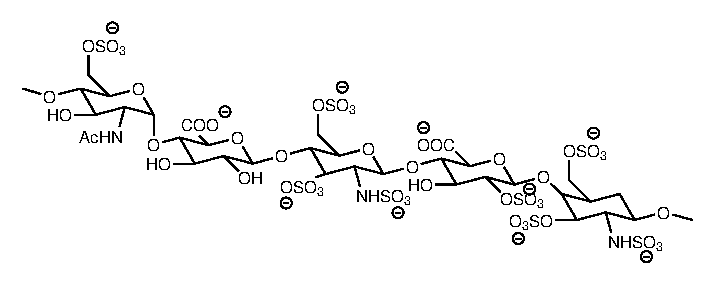
\includegraphics{Figures/heparin_pentasaccharide.eps}}
\caption{Pentasaccharide sequence which gives heparin its characteristic anticoagulant properties. Adapted from \cite{Bromfield2013HeparinApplications,Peterson2009DesignApproach}}
\label{heparin_pentasaccharide}
\end{figure}

There are two separate pathways which control coagulation, as shown in Figure \ref{coagulation_cascade}, “extrinsic” (tissue factor pathway) and “intrinsic” (contact activation pathway), and a pathway which is common to both; unsurprisingly called the common pathway.\textsuperscript{\cite{Sabir2014OralFibrillation}}
\begin{figure} [ht!]
\centering{
\includegraphics{Figures/coagulation_cascade.eps}}
\caption{The 3 pathways in the coagulation cascade. Roman numerals are used to identify coagulation factors.
Adapted from \cite{Palta2014OverviewSystem.,Peters2013UtilizationTherapeutics,Hirsh2001MechanismHeparin}}
\label{coagulation_cascade}
\end{figure}
\newline
Heparin works by binding to both an enzyme inhibitor known as antithrombin III and if the heparin chain is more than 18 pentasaccharides long, it binds to factor Xa as well.\textsuperscript{\cite{Hirsh2001MechanismHeparin}} This then prevents prothrombin from being converted into thrombin, and interferes with the function of the so-called “common” pathway; a blood clot cannot be formed. 

\subsection{Medical Applications of Heparin Sulfate}
Heparin sulfate finds itself used for a variety of reasons within medicine, most notably as an anticoagulant during major surgery, whether this be during the insertion of a stent to hold cardiac arteries open after a myocardial infarction or during major transplant surgery. In this case, heparin is used to prevent coagulation inside the extracorporeal circuit.\textsuperscript{\cite{BritishMedicalAssociation.2017BNF2017.}} 
\newline
It also finds use as prophylactic treatment for deep vein thrombosis (DVT), even though heparin sulfate cannot break down clots which have already formed, and is used as an additive in the green topped vacutainer vials used in phlebotomy where heparin is used as its lithium salt to prevent coagulation of blood samples.\textsuperscript{\cite{BritishMedicalAssociation.2017BNF2017.}}

\subsection{Issues Associated with Heparin Use}
There are a variety of well-known issues with using heparin as an anticoagulant.
Firstly; as already mentioned, a high proportion of heparin lacks the necessary pentasaccharide sequence that provides its characteristic anticoagulant activity. This causes issues when it is necessary that the total heparin load\footnote{Heparin load - total amount of heparin administered. Includes both the active and inactive parts of heparin.
\newline
Heparin dose - total amount of active heparin. Measured in international units (IU).} is known.   Quantifying heparin levels is typically achieved during surgery \textit{via} an activated clotting time assay. These clotting time based assays are very good at measuring the amount of heparin that is active, but cannot easily determine the heparin load. 
\newline
Secondly, there is an issue with the clotting time based assays themselves. They are slow, and importantly, cannot be performed in situ.\textsuperscript{\cite{Bromfield2013HeparinApplications}} 
\newline
Finally, it is known that not all heparin preparations are the same. Differences arise from the origin of the heparin preparation i.e. bovine vs porcine, in terms of both the structure of the isolated heparin, and its activity.\textsuperscript{\cite{Mulloy2015PharmacologyDrugs}} Bovine sourced heparin can be isolated from both lung and intestinal tissue, whilst porcine sourced heparin is exclusively from intestinal tissue.\textsuperscript{\cite{Tovar2013BovineHaemodialysis.}} Both forms of heparin are often used as if they were indistinguishable in their structure and activity, despite the fact heparin of porcine origin has much higher activity, and hence smaller quantities can be used.  Heparin is provided clinically simply in terms of 'units of activity', with little attention paid to the inactive material. 
\newline
It is important to note that since the 1980's, all licensed heparin products used within the European Union and USA have been of porcine origin, due to the possibility of transmitting variant Creutzfeld-Jakob disease (vCJD) via heparin of bovine origin.\textsuperscript{\cite{Mulloy2015PharmacologyDrugs}}  

\section{Protamine Sulfate}
Protamine sulfate is an arginine-rich cationic peptide of ill-defined structure, often derived from salmon sperm, that is used medically to reverse the anticoagulant behaviour of heparin.\textsuperscript{\cite{Bromfield2013HeparinApplications,Balhorn2007TheProteins}}
Due to issues with the clotting time based assays outlined above, dosing protamine for use as a heparin rescue agent at the end of surgery, is difficult. Dose too much, and the patient will clot too well, potentially be at risk of blood clots forming as well as increasing the risk of developing side effects from protamine sulfate, dose too little and the patient will not clot sufficiently well that healing can begin.
\newline
Finally, the way that protamine itself binds heparin is also problematic, as it makes no distinction between active and inactive parts of heparin, which then leads to larger doses of protamine sulfate being necessary, and hence a greater likelihood of side effects being experienced. Up to 10\% of all those given this rescue agent will have some form of side effect, and those most at risk include those who have had previous treatment with protamine sulfate, insulin-dependent diabetics who take long acting forms containing protamine sulfate, those with a fish allergy and men who are infertile.\textsuperscript{\cite{Bromfield2013HeparinApplications,BritishMedicalAssociation.2017BNF2017.}} 

\subsection{Binding of Protamine Sulfate to Heparin}
The use of protamine sulfate as a rescue agent for heparin is fraught with issues: from the difficulty in dosing, due to the non-selective way it binds to heparin, to the side effect known as heparin rebound first noted by Kolff \textit{et al.} in 1956, where not enough protamine sulfate has been dosed, and as heparin unbinds from plasma proteins, a de-coagulation event and bleeding occurs.\textsuperscript{\cite{Kolff1956DisposableMedicine}} Despite this, protamine sulphate remains the only rescue agent for heparin to gain clinical approval. 
\newline
The binding of protamine sulfate to heparin, which abolishes its anticoagulant ability is based on electrostatic binding. Clearly this opens the possibility of developing systems which can exhibit more selective heparin binding, and potentially only bind to the active polysaccharide sequence, whilst avoiding the side effects associated with the current use of protamine sulfate. 

\section{DNA}
Deoxyribonucleic acid (DNA) contains a varying composition of 4 specific nucleotide bases (guanine, cytosine, adenine and thymine), as well as deoxyribose sugars connected by phosphodiester bonds forming the characteristic sugar-phosphate backbone of DNA.\textsuperscript{\cite{Hamilton2012NaturalBinders}} Hydrogen bonding between these nucleotide bases forms Watson-Crick base pairs (G with C and A with T) and leads to the characteristic double stranded helix known as B-DNA.\textsuperscript{\cite{Voet2011Chapter5}} This B-DNA form has a repeating pattern of wide major grooves, and narrower minor grooves on its surface, in which a variety of molecules can bind (Figure \ref{B-DNA_structure}). 
\begin{figure} [ht!]
\centering{
\includegraphics[scale=0.75]{Figures/DNA.png}}
\caption{The repeating pattern of major and minor grooves in B-DNA. From \cite{Nelson1987TheImplications}.}
\label{B-DNA_structure}
\end{figure}
\newline
Heparin sulfate however, is very different to DNA. It is a linear oligosaccharide of varying composition and length, and as such, adopts a very different secondary structure to DNA, instead choosing to form long chains.
Even though there are differences between the roles that DNA and heparin sulfate play within the human body, one being an incredibly important molecule with a well defined, regular structure, which contains all the genetic material necessary for any given living organism; the other being of irregular polymeric structure and used as an anticoagulant, there are similarities between them. Both heparin with its sulfate groups and DNA with phosphate groups are biologically relevant polyanionic molecules.\textsuperscript{\cite{Mulloy2015PharmacologyDrugs}}
\newline
There has been much research into DNA, due to the interest in gene therapy for a variety of congenital disorders not limited to, but including Cystic Fibrosis.
In contrast, there has been comparatively little study of the binding of heparin sulfate to protamine, and even less which attempts to compare and contrast the two.  
\subsection{Binding DNA and Gene Therapy}
%binding to DNA
Small molecules can either interact with DNA in a covalent, or non-covalent fashion. Covalent binding to DNA results in a permanent change in the shape of the DNA binding site, whilst non-covalent interactions are often reversible.\textsuperscript{\cite{Hamilton2012NaturalBinders}} These potentially reversible non-covalent interactions include intercalation between base pairs, electrostatic interactions with the phosphodiester backbone of DNA or interactions with the functional groups of the base pairs in either the major or minor grooves (Table \ref{DNA_binders}).\textsuperscript{\cite{Hamilton2012NaturalBinders,Tuite1997EffectsDichroism}} 

\begin{table}[ht!]
\centering
\caption{A selection of major/minor-groove binders and DNA intercalating agents}
\begin{tabular}{l|l|l}
\textbf{Major-groove binder} &\textbf{Minor-groove binder} &\textbf{Intercalating agent} \\
\hline
Methyl Green& Distamycin A & Ethidium Bromide\\
& & Methylene Blue\\
\end{tabular}
\label{DNA_binders}
\end{table}

It has also been shown by Broggini \textit{et al.}, that the two grooves do not behave independently, as binding distamycin A into the minor-groove leads to interference with the major-groove binding of various regulatory proteins.\textsuperscript{\cite{Broggini1989DistamycinsElements.}}

Gene therapy has the potential to cure cancer, and genetic disorders of both congenital and acquired origin.  For this to be possible, it requires nucleic acids to be transported across the cell membrane by some form of vector, as DNA cannot translocate across cell membranes unaided.\textsuperscript{\cite{Ghosh2008EfficientNanoparticles}} Viral vector methods work well, but there are significant safety concerns with the use of these methods for gene delivery, e.g.  the ability of the vector to revert to wild type, or replication competent virions, the risk of inherent immunogenicity as well as the vector causing an inflammatory response.\textsuperscript{\cite{Ghosh2008EfficientNanoparticles,Kim2016PolycationsApplications}} 

A variety of synthetic vectors have been developed, often based upon polymers, dendrimers or liposomes.  These synthetic vectors avoid some of the issues associated with viral methods, but often suffer from poor loading of genetic material. It is also often difficult to achieve nuclear uptake after cell penetration. It also must be noted that a relatively high molecular weight of the synthetic vector is necessary to lead to effective condensation of DNA, and this high molecular weight often leads to these synthetic systems being cytotoxic.  
There are a variety of cationic polymers which are capable of binding DNA. These include poly-L-lysine (PLL), polyethyleneimine (PEI) as well as PAMAM dendrimers. PLL has been used as a DNA delivery agent for over 20 years due to its relative biocompatibility, and the ease at which it can be degraded by cells.\textsuperscript{\cite{Zauner1998Polylysine-basedDelivery}}  

Cationic lipids have also been used to deliver DNA inside cells. They were first pioneered by Felgner \textit{et al.} in the late 1980's and after further studies, several of these cationic lipid systems are now commercially available.\textsuperscript{\cite{Felgner1987Lipofection:Procedure,Malone1989CationicTransfection}}  
DOTMA (N-[1(2,3-dioleyloxy)propyl]-N,N,N-trimethylammonium chloride) is now sold under the trade name Lipofectin, and DOSPA (2,3-dioleyloxy-N-[2(sperminecarboxido)ethyl]-N,N,-dimethyl-1-propanaminium trifuloroacetate) is sold as Lipofectamine.\textsuperscript{\cite{LipofectinTransfectionReagent-ThermoFisherScientificHttps://www.thermofisher.com/order/catalog/product/18292037,LipofectamineReagent-ThermoFisherScientificHttps://www.thermofisher.com/uk/en/home/brands/product-brand/lipofectamine.html}} 

There are a variety of challenges synthetic vectors must overcome before they can be used as viable transfection methods; these include effective complexation and condensation of the DNA, cellular uptake, and more importantly, endosomal escape as well as nuclear translocation.\textsuperscript{\cite{Ghosh2008EfficientNanoparticles}} Without successful endosomal escape and translocation, the DNA will be transported inside the cell, but not reach the nucleus. 
More recently, CRISPR (Clustered Regularly Interspaced Short Palindromic Repeat)/Cas9 (CRISPR associated gene 9) has been employed as a potential method of genetic delivery. However, once the DNA has been delivered, the CRISPR genes stay behind in the host cell. This has the potential to cause unwanted gene editing - clearly problematic in therapeutic applications, and there is the possibility of immunogenic responses in the host.\textsuperscript{\cite{Mout2017DirectEditing}} 
Various strategies of using CRISPR for genetic editing have been reported in the literature, but they often result in endosomal entrapment of Cas9 and/or single guide RNA (sgRNA).\textsuperscript{\cite{Sun2015Self-AssembledEditing,Zuris2015CationicVivo}}

\subsection{Gene Delivery in Cystic Fibrosis}
Cystic Fibrosis (CF) is a congenital genetic disorder where sufferers receive a faulty copy of the gene which codes for the CFTR (Cystic Fibrosis Transmembrane Conductance Regulator) protein from both parents.
The CFTR gene was not identified until 1989, since then more than 2000 different mutations have been identified.\textsuperscript{\cite{Castellani2017CysticView} } These mutations can be sorted into 6 different classes, based on the type of malfunction within the CFTR protein. 
These mutations differ in the organs that are involved, with lung involvement being most variable. They also differ in the severity of the disorder and the rate of progression. However, these classes cannot be used to predict an individual's outcome with Cystic Fibrosis, as such, these classes are of more use within clinical trials. 

Several theories exist as to how a malfunctioning CFTR protein leads to the symptoms associated with CF.  The most accredited theory states: malfunctioning CFTR protein leads to a lack of water in pericilliary fluid and results in abnormally dense mucus. This mucus is then difficult for the cillia to clear. This faulty protein then causes an increased inflammatory response and decreased activity of natural defense mechanisms, which unsurprisingly facilitates the development of  the symptoms traditionally associated with the disorder, such as repeated lower respiratory tract infections. 
\newline
Research is currently focused on treatments for restoring the function of the CFTR protein, some of which have shown promising results in clinical trials.\textsuperscript{\cite{Castellani2017CysticView}} One way of achieving this would be through intracellular delivery of a correctly functioning copy of the affected gene.  

As genetic therapy advances ever closer towards clinical application, several clinical trials have assessed the potential benefits for a variety of genetic disorders.  A small double-blind study involving 140 CF sufferers was undertaken in 2012 to prove the viability of using inhaled gene-liposome complexes as a potential treatment for some of the respiratory symptoms associated with Cystic Fibrosis.\textsuperscript{\cite{Alton2015RepeatedTrial}} The results show that this certainly isn't a cure for the disorder, but did prevent some decline in lung function. It was noted that further clinical studies of gene delivery vehicles for CF were urgently needed, as this trial did not select participants with a particular type of CFTR mutation, nor could it explain why one group of patients - particularly those with a predicted FEV\textsubscript{1} (forced expiratory volume in 1 second) of <69.2 \% had a greater response than those who were less unwell. 
\section{Multivalent Interactions and Self-Assembly}
In order to bind nanoscale polymeric structures such as heparin or DNA, it is necessary to marshal multiple non-covalent interactions - so called multivalency. As outlined above, systems which can do this may have potential applications in both heparin rescue and/or gene delivery. The cationic polymers and dendrimer systems discussed previously, have been shown to function as potential protamine sulfate mimics, but their toxicity makes medical application unlikely. Also, for even the most simple, first-generation (G1) dendrimers, they often have complex, multi-step syntheses.\textsuperscript{\cite{Rodrigo2011Self-AssemblingBinding}} Due to the difficulty of constructing a covalent array of ligands to bind to a specific target, there has been increasing interest in using self-assembly to organise the multivalent ligands. 

The phenomenon of self assembled multivalency was first reported in 1992 by Whitesides and coworkers in a paper outlining self assembled sugars that bound better to a sugar binding protein than their monovalent counterparts. The polyvalent system is more efficient than the monovalent form – not a surprise considering a central idea of supramolecular chemistry is that polyvalency is superior to monovalency in terms of both efficiency and affinity of binding.\textsuperscript{\cite{Kingery-Wood1992TheGangliosides}} 

\subsection{Self Assembled Multivalency (SAMul)}
Barnard and Smith went on to define self-assembled multivalency in a key review.\textsuperscript{\cite{Barnard2012Self-AssembledBinding}} They defined the phenomenon as relying on small molecules being self assembled into a larger nanostructure, which has the ability to form a multivalent binding array. They noted that this method has a variety of advantages including:
\begin{itemize}
\item spontaneous simple assembly, 
\item well-defined low-molecular-weight building blocks suitable for clinical approval
\item ability to assemble different active components into a single nano-structure
\item simple or triggered disassembly/degradation.\textsuperscript{\cite{Bromfield2013HeparinApplications,Barnard2012Self-AssembledBinding}}
\end{itemize}
The advantages of these SAMul systems come about for a variety of reasons. A carbon chain is often used as the hydrophobe to drive self-assembly. The spontaneous assembly arises from a fine balance between hydrophobic and hydrophilic components of the molecule.   
\newline 
Triggered bond cleavage of these systems is possible by inserting, for example, an ester group between the hydrophobic tail and hydrophilic binding group. Ester groups are well known to degrade under biological conditions. When the ester undergoes hydrolysis, the molecule breaks apart and self assembly of the system is no longer possible. Once the molecule loses the ability to self assemble, its binding ability is then "switched off". 
%insert cartoon of self-assembly here
\newline
Degradation and disassembly then also limits the biopersistance of the molecule and helps with issues of toxicity that can be present with polymeric multivalent binding systems.\textsuperscript{\cite{Rodrigo2011Self-AssemblingBinding, Barnard2012Self-AssembledBinding}}

\newpage
\section{Potential Protamine Sulfate Mimics}
A variety of different research groups have attempted to synthesise a biologically compatible protamine sulfate mimic, and several alternate approaches have been used. These include:
\begin{itemize}
\item  cationic polymers and dendrimers
\item protein based heparin binders
\item small molecules
\item Self-Assembled Multivalency (SAMul)
\end{itemize}
\subsection{Cationic Polymers and Dendrimers}
A popular approach for developing synthetic protamine sulfate mimics is to base the structure on a large cationic compound which binds heparin via multiple electrostatic interactions. Both multivalent cationic polymers and dendrimers (branched macromolecules of regular, well defined structure) have been used, and can achieve high binding affinity to heparin. However, cationic polymers tend to be biopersistant and hence toxic – this can be a problem.\textsuperscript{\cite{Rodrigo2011Self-AssemblingBinding, Barnard2012Self-AssembledBinding}}
It has been shown by Fr\'{e}chet \textit{et al.} that neutral, low generation dendrimers are water soluble, and likely to be more suitable for medical applications.\textsuperscript{\cite{PadillaDeJesus2002PolyesterEvaluation}}

\begin{figure} [ht!]
\centering
\includegraphics[scale=1.0]{Figures/PAH_structure.eps}
\caption{Structure of Poly(allylamine hydrochloride)}
\label{PAH_structure}
\end{figure}

Functionalised poly(allylamine hydrochloride) (PAH) derivatives have  been trialled as potential protamine sulfate mimics. Naturally derived polymers have issues with batch-to-batch variation, and hence, it was argued that a synthetic polymer is more appealing.\textsuperscript{\cite{Kaminski2014NewReversal}} Kami\'{n}ski \textit{et al.} chose to use a poly(allylamine hydrochloride) backbone as it already finds a variety of uses within medicine and therefore, it was possible that a functionalised derivative of this would also be biologically compatible. The scaffold was then functionalised with arginine groups, to enable it to bind heparin in the same manner as protamine sulfate.  Azure A displacement assays showed that the dose of this arginine-functionalised PAH derivative required to neutralise a 1 mg dose of heparin was less than half that of protamine sulfate (0.46 mg).\textsuperscript{\cite{Kaminski2014NewReversal}} Cytotoxicity studies were also performed and showed that the functionalised PAH derivative was less cytotoxic than the PAH scaffold alone. 

\begin{figure} [ht!]
\centering
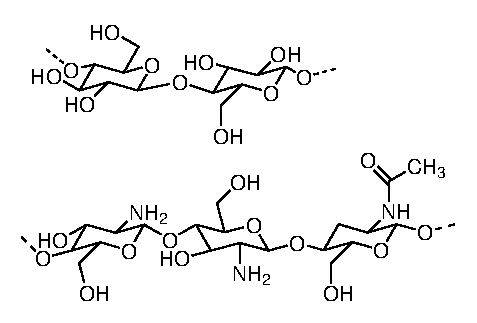
\includegraphics[scale=1.0]{Figures/dextran+chitosan_structure.eps}
\caption{Top: structure of dextran. \newline
Bottom: structure of chitosan.}
\label{dextran+chitosan_structure}
\end{figure}
Kami\'{n}ski \textit{et al.} also developed cationic derivatives of chitosan and dextran. \textit{ In vitro} and \textit{in vivo} testing of these compounds was positive.\textsuperscript{\cite{Kaminski2014NewReversal}}  Notably, no immunogenic response was shown, and they act as effective heparin antidotes. However, in rat models, it has been shown that these compounds are not completely free of side effects. The chitosan derivatives interact with erythrocytes while dextran derivatives cause hypotension - like protamine sulfate.\textsuperscript{\cite{Kaminski2014NewReversal}} 

Dex40-GTMAC3 is a functionalised dextran derivative with an average molecular weight of 40 kDa, and functionalised with glycidyltrimethylammonium chloride (GTMAC) at a ratio of 0.65 GTMAC groups per glucose unit.\textsuperscript{\cite{Sokolowska2016TheHeparin}} Recently published work shows that these functionalised dextrans are non-toxic, biodegradeable and function well as protamine sulfate mimics.\textsuperscript{\cite{Kalaska2015NonclinicalHeparin}} Toxicology studies on rats have shown that there is rapid renal clearance of the drug, with plasma concentration falling to less than half of that administered after 10 minutes, and little in terms of tissue accumulation.\textsuperscript{\cite{Kalaska2015NonclinicalHeparin}}  Therefore, this dextran derivative is much better tolerated than protamine sulfate. However, the researchers are aware much more testing needs to be done before this functionalised dextran derivative can enter clinical trials. 

\subsection{Proteins, Peptides and Peptoids}
Ford, Hamza and Rabenstein used N-substituted glycine peptoids, generated systematically by solid-phase synthesis.\textsuperscript{\cite{Ford2013DesignPeptoids}} The use of substiuted peptoids (Figure \ref{peptide_vs_peptoid}) rather than peptides, leads to several advantages, particularly when considering the use of these molecules as potential drug candidates. Peptoids are resistant to proteases unlike peptides and are better able to pass through biological membranes. Most importantly as potential protamine sulfate mimics, they do not trigger an immunogenic response. 
\begin{figure} [ht!]
\centering
\includegraphics{Figures/peptide_vs_peptoid.eps}
\caption{Generic tetrapeptide (top) and generic tetrapeptoid (bottom). Adapted from \cite{Ford2013DesignPeptoids}}
\label{peptide_vs_peptoid}
\end{figure}

It was discovered by Carson and coworkers that there is a naturally occurring heparin interacting protein (HIP) present in human uterine epithelial cells, and subsequently the heparin binding domain of this protein was sequenced.\textsuperscript{\cite{Rohde1996CellLines.,Liu1996CDNALines.}} 
In 2006, two synthetic analogues (Figure \ref{HIPAP_structure}) of this heparin interacting protein were synthesised by Wang and Rabenstein.\textsuperscript{\cite{Wang2006Interactionsup/sup}}

\begin{figure} [h!]
\centering
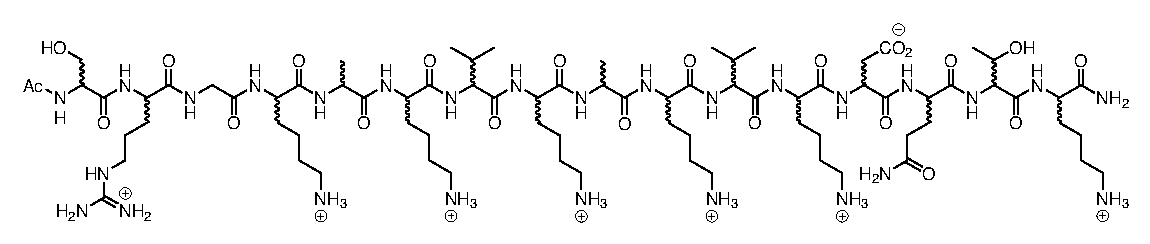
\includegraphics[scale=0.85]{Figures/HIPAP_structure.eps}
\caption{Structure of HIPAP. Adapted from \cite{Wang2006Interactionsup/sup}.}
\label{HIPAP_structure}
\end{figure}

These heparin interacting protein analogue peptides (HIPAP) differed from each other only in the chirality of the amino acids that were used. One used purely the endogenous L-form, and the other, purely D-forms of the amino acids.  It was noted that both L-HIPAP and D-HIPAP are capable of binding heparin, neutralising its anticoagulant activity, and that they are equally effective. It was also shown that the spatial arrangement of the six lysines and the one arginine residue play an important role in the heparin binding ability, as a scrambled version of this peptide did not effectively bind heparin. These observations suggest that charge density and spacial organisation of charge, not chirality, are the most dominant forces in these heparin-binding systems. 

\subsection{Small Molecule-Based Heparin Binders}
There have been several small molecule based heparin binders reported in the literature. Key examples include delparantag, ciparantag and functionalised calix[8]arenes.\textsuperscript{\cite{Bromfield2013HeparinApplications}} 
\begin{figure} [h!]
\centering
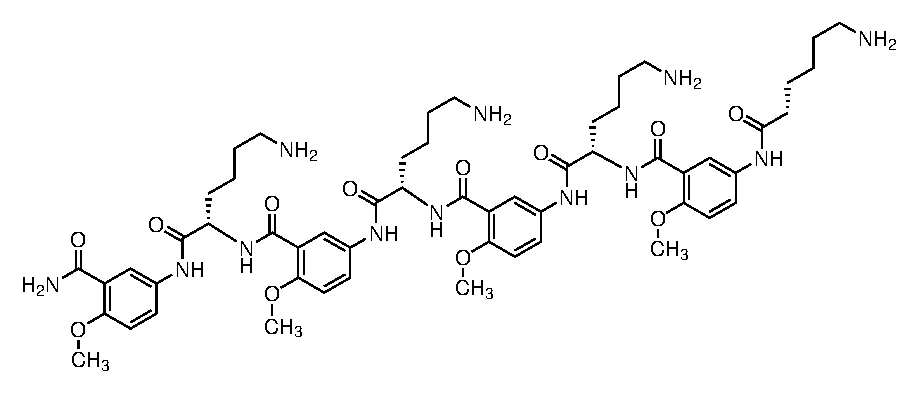
\includegraphics[scale=0.85]{Figures/delparantag_structure.eps}
\caption{Structure of Delparantag. Adapted from \cite{Mahan2014AAgents}.}
\label{delparantag_structure}
\end{figure}

Delparantag (PMX-60056) is a novel salicylamide-derived small molecule with a molecular weight of 1,126 Da.\textsuperscript{\cite{Mahan2014AAgents}} It was designed to interact with the pentasaccharide sequence and prevent the interaction with antithrombin III. It underwent several phase IB/II trials and showed promising results, notably being one of the few potential protamine sulfate mimics capable of full reversal of the effects of both unfractionated heparin (UFH) and  low molecular weight heparins (LMWH).\textsuperscript{\cite{Mahan2014AAgents,Kuziej2010InDerivative}}
However, the trial was halted and then terminated in May 2012 due to participants developing hypotension on administration of Delparantag.\textsuperscript{\cite{ReversalClinicalTrials.gov}} No further trials are currently in progress.

\begin{figure} [h!]
\centering
\includegraphics[scale=0.85]{Figures/ciraparantag_structure.eps}
\caption{Structure of ciraparantag.}
\label{ciraparantag_structure}
\end{figure}

Ciraparantag (PER977) (Figure \ref{ciraparantag_structure}) is another synthetic, water soluble cationic molecule designed specifically to bind to both LMWH and UFH by non-covalent hydrogen bonding and electrostatic interactions.\textsuperscript{\cite{Ansell2014UseEdoxaban}} It is currently undergoing phase II trials, and if shown to be both safe and effective, it could become the first broad-spectrum rescue agent for novel oral anticoagulants (NOAC). 

It has already been shown that ciraparantag restores baseline haemostasis within 30 minutes of administration, is well tolerated by patients, and does not interact with several other drugs.\textsuperscript{\cite{Ansell2014UseEdoxaban,Ansell2016CiraparantagHeparin}} The interaction of ciraparantag was assessed with the anticonvulsives lamotrigine and carbamazepine (the latter also finding itself used as a mood stabiliser in bipolar disorder), and several cardiac medications including the antiplatelet drug clopidogrel, which is useful in the case of patients undergoing polypharmacotherapy.\textsuperscript{\cite{BritishMedicalAssociation.2017BNF2017.,Laulicht2013AntidoteEdoxaban}}

\begin{figure} [h!]
\centering
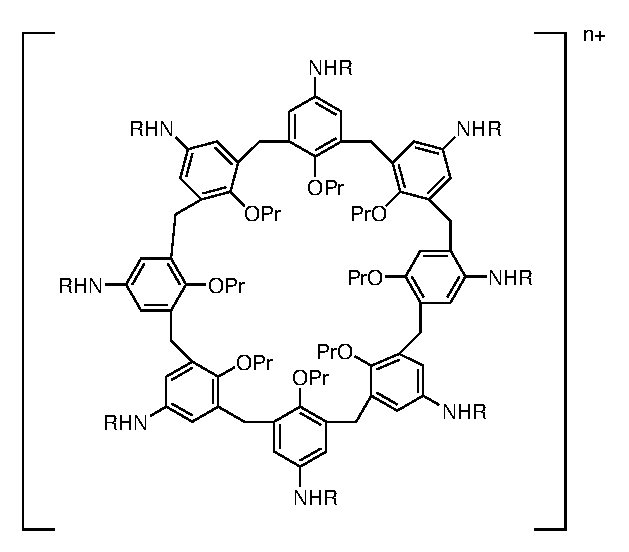
\includegraphics[scale=0.75]{Figures/calix_8_arene.eps}
\caption{Structure of the functionalised calix[8]arene synthesised by Cunsolo \textit{et al.} Adapted from \cite{Mecca2006PolycationicHeparin}.}
\label{calix[8]arene_scaffold}
\end{figure}

Functionalised calix[8]arenes were reported by Cunsolo \textit{et al.} in 2006 as potential protamine sulfate mimics. The calix[8]arene scaffold (Figure \ref{calix[8]arene_scaffold}) was chosen due to its conformational adaptability. Two different functionalised calix[8]arene scaffolds were synthesised in order to probe the effect of charge density on the binding affinity towards heparin. It was also hypothesised by the researchers that the flexibility of both the calix[8]arene and heparin would improve binding affinity. 
On comparison of the results for binding heparin to protamine sulfate, this was shown to be true, as the rigid structure of protamine negatively affected the rate of complexation.\textsuperscript{\cite{Mecca2006PolycationicHeparin}} 
\newpage
It was also shown that the rate of complexation is affected more strongly by the adaptability and flexibility of the host:guest complex, than by simple charge density. 

\subsection{Self-Assembled Multivalency (SAMul)}
Self-assembled multivalency (SAMul) has also been employed as a method by which novel protamine sulfate mimics could be produced. This approach is very different to that used by Ford and Rabenstein, and has a variety of advantages which have already been outlined above. Particularly useful is the ability to combine several components into a single structure, and the possibility for simple or triggered disassembly. 

The use of SAMul in the development of nanoscale self-assembling heparin binders was first reported in the literature by Campo-Rodrigo, Barnard \textit{et al.} in 2011.\textsuperscript{\cite{Rodrigo2011Self-AssemblingBinding}} This paper showed that a self-assembling dendron (Figure \ref{C22-G1_structure}) could be used to bind heparin when functionalised with amines, that are protonated at physiological pH, and a hydrophobic group is necessary to drive the self-assembly. This implies that at least part of binding the self-assembled nanoscale interface to heparin has an electrostatic component. However, it was also noticed by the researchers that the synthesis of this system was certainly not facile, and that significant further work was necessary to probe the ability of this dendron to disassemble and degrade, as it was already known that dendrimers are biopersistent and can be toxic.
\begin{figure} [h!]
\centering
\includegraphics[scale=0.75]{Figures/G1_structure.eps}
\caption{Structure of the C22-G1 self-assembling dendron synthesised by Campo-Rodrigo \textit{et al.} Adapted from \cite{Rodrigo2011Self-AssemblingBinding}.}
\label{C22-G1_structure}
\end{figure}

Further work was carried out on this system by Bromfield \textit{et al.} to probe whether this self-assembling "pseudo-dendrimer" was still as effective at binding heparin in biologically competitive media.\textsuperscript{\cite{Bromfield2014NanoscaleMedia}} The binding assays in the Campo-Rodrigo paper were only performed in phosphate buffered saline (PBS), which bears little resemblance to human serum in terms of the electrolytes that it contains. Therefore, the assays to assess heparin binding were performed in a solution of 150 mM NaCl and 10 mM Tris-HCl. It was shown that C22-G1 still self-assembles in solution, and the increased salt concentration increases the size of the self-assembled micelle. This is unsurprising as increasing the ionic strength of a solution is known to increase both the screening of surface charge and the impact of the hydrophobic effect.\textsuperscript{\cite{Bromfield2014NanoscaleMedia}} This then leads to a greater number of individual molecules being included in the self-assembled micelle, hence increasing its diameter.

Bromfield then went on to assess the self-assembly of C22-G1 in human serum. Human serum contains all the electrolytes and blood components found within human blood, with the exception of those involved in blood clotting.\textsuperscript{\cite{Bromfield2014NanoscaleMedia}} It was hoped that if this system could still function in human serum, and be a more effective heparin binder than the currently utilised protamine sulfate, then medical application of these self-assembling pseudo-dendrimers could become reality.  Unfortunately, the results showed that C22-G1 becomes less effective as a heparin sulfate binder in human serum, with its CE\textsubscript{50} value rising from 0.28 to 0.96. However, the compound was demonstrated in some clotting assays to still function optimally in human plasma.\textsuperscript{\cite{Bromfield2014NanoscaleMedia}} 

The effect of flexibility on binding self-assembling nanoscale interfaces to heparin and/or DNA, was then studied. Fechner, Albanyan \textit{et al.} modified only the binding group and kept the hydrophobic component of their systems the same.\textsuperscript{\cite{Fechner2016ElectrostaticBinding}} This work showed that certain binding groups had a greater binding affinity to heparin/ DNA than others (Figure \ref{SPM_vs_SPD}). 
\begin{figure} [ht!]
\centering
\includegraphics[scale=0.9]{Figures/SPM_vs_SPD.eps}
\caption{The differences in structure between spermidine (above) and spermine (below). From \cite{Fechner2016ElectrostaticBinding}.}
\label{SPM_vs_SPD}
\end{figure}

The self-assembling interfaces with spermidine ligands had a greater affinity for heparin, whilst those with spermine ligands had greater affinity for DNA. It was also noted that DNA appears to be a “shape-persistent” polyanion, which will attempt to organise the SAMul assembly that it is presented with. In contrast, Heparin is a “adaptive” polyanion, which changes itself in response to the SAMul binding surface.\textsuperscript{\cite{Fechner2016ElectrostaticBinding}} These results also strongly agree with the arguments made by Cunsolo \textit{et al.} that the flexibility of heparin also plays a key role in binding.\textsuperscript{\cite{Mecca2006PolycationicHeparin}}

Over the past 6 years, the structure of these self-assembling nanoscale heparin binders has been repeatedly modified, and is now very different to the structure originally used by Campo-Rodrigo and Barnard.\textsuperscript{\cite{Rodrigo2011Self-AssemblingBinding}} It is no longer a first generation dendron, but a small, discrete molecule capable of self assembly. These molecules now consist of a hydrophobic carbon chain, used to encourage the molecule to self-assemble in aqueous media, and a binding group displayed on the outside of the self-assembled micelle, which is positively charged at physiological pH. 

More recently, work has been published exploring the effect of modifying the hydrophobic carbon chain on binding of these nanoscale systems to both heparin and DNA. Vieira, Liljestr\"om \textit{et al.} used C14-DAPMA, C16-DAPMA and C18-DAPMA to assess the effect of changing hydrophobic chain length on binding to heparin sulfate.\textsuperscript{\cite{Vieira2017EmergenceHeparin}}  It was noted that altering hydrophobic chain length had an effect on the solubility of these nanostructures, as C18-DAPMA was poorly soluble in PBS buffer.  The measured \textzeta - potentials also highlighted the effect changing the length of the carbon chain has on the ability of the molecule to self-assemble. The greater the \textzeta-potential, the greater the driving force required for self assembly, and this is seen to increase with increasing chain length.  Albanyan, Laurini \textit{et al.} also modified the hydrophobic chain by changing the number of double bonds along its length.\textsuperscript{\cite{Albanyan2017Self-AssembledLigands}} The self-assembly of these structures was quantified using Nile Red assays, and it was shown that increasing numbers of double bonds increased both critical micelle concentration, as well as the diameter of the self-assembled micelles. Surprisingly, results also showed that altering the number of double bonds in the carbon chain alters the selectivity of these systems towards both DNA and heparin. C18-1 shows a strong preference towards heparin binding relative to that for DNA, whilst the results are the reverse for C18-3. This is believed to occur because of the degree of preorganisation imparted into the molecule by increasing numbers of cis double bonds and the "shape-persistant" behaviour of DNA. 

\begin{figure} [ht!]
\centering
\includegraphics{Figures/C16-Gly-Lys.eps}
\caption{The self-assembling nanoscale binder developed by Chan et al. From \cite{Chan2016ChiralBinding}.}
\label{C16-Gly-Lys}
\end{figure}

Finally, it has been noted that these newer self-assembling nanoscale binders can also display chiral selectivity (Figure \ref{C16-Gly-Lys}).  It is known that a SAMul binder composed of only palmitic acid and a L/D-lysine binding group will bind to heparin and DNA, but display no chiral preference.\textsuperscript{\cite{Chan2016ChiralBinding}} On insertion of an amino acid spacer group, in this case glycine, chiral selectivity was "switched on".  This chiral selectivity is useful as it enables us to tune the selectivity of the SAMul interface towards a particular biological polyanion. Binding assays show that C\textsubscript{16}-Gly-D-Lys has a much improved affinity for DNA compared to its analogous L-lysine containing counterpart, and it was suggested that the insertion of the glycine spacer group enables the molecule to "better express its chirality", as the insertion of the glycine spacer group modifies both the shape and polarity.\textsuperscript{\cite{Chan2016ChiralBinding}} It was also suggested that the addition of a glycine spacer leads to additional hydrogen bonding sites and potentially modifies the binding between the SAMul system and binding partner.  As a consequence, it is believed that this chiral selectivity may remain, if the spacer group is changed from glycine to another chiral amino acid. 

Using self-assembly to create systems capable of inhibiting the function of heparin sulfate has not only been explored by Smith and coworkers. In 2014, DeGrado \textit{et al.} published a paper in which the phenomenon of self-assembly was applied to create heparin-binding foldamers.\textsuperscript{\cite{Montalvo2014DeInteractions}} Foldamers are non-biological sequence specific polymers of a defined length, which also possess well defined secondary and tertiary structures. They are often used to assess the folding and function of various biomacromolecules and have been used more recently to inhibit protein-protein interactions. The foldamers used by DeGrado \textit{et al.} were based on a repeating pattern of lysine and 5-amino-2-methoxy-benzoic acid (Sal) units (Figure \ref{Lys-Sal_foldamer}).

\begin{figure} [ht!]
\centering
\includegraphics{Figures/Lys-Sal_foldamer.eps}
\caption{Repeating Lys-Sal unit in the heparin-binding foldamers used by DeGrado \textit{et al.} From \cite{Montalvo2014DeInteractions}.}
\label{Lys-Sal_foldamer}
\end{figure}

The results showed that the binding affinity of these Lys-Sal foldamers did not depend on the chirality of the lysine side chains, and that like the nanoscale SAMul systems developed by Chan \textit{et al.}, self-assembly of the foldamer is necessary before heparin binding can take place.\textsuperscript{\cite{Chan2016ChiralBinding,Montalvo2014DeInteractions}}

\section{Designing Novel Nanostructures}
The novel molecules in this work (Figure \ref{C16-Ala-Lys_family})
were designed in such a way that they have low molecular weight - as it is known these are more likely to achieve approval for medicinal use.\textsuperscript{\cite{Bromfield2013HeparinApplications}}
The lysine binding group has been chosen due to its ubiquitous appearance in nature, particularly within polyanionic binding proteins, and for its ability to bind heparin, as the amino acid is positively charged at physiologically relevant pH.\textsuperscript{\cite{Bromfield2015HeparinNanostructures}}
\begin{figure} [h!]
\centering
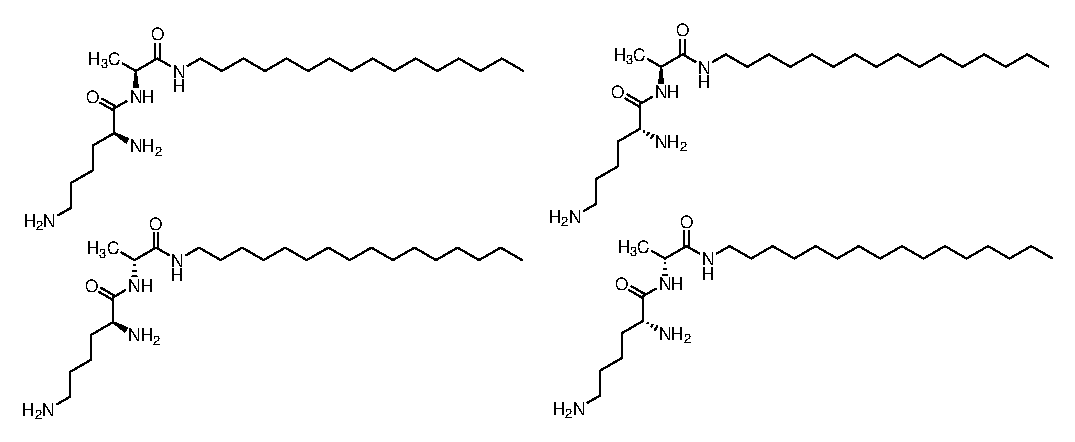
\includegraphics[scale=0.9]{Figures/C16-Ala-Lys_family.eps}
\caption{ The novel self-assembling heparin binders synthesised in this work. \newline
L-R Top row: C\textsubscript{16}-L-Ala-L-Lys, C\textsubscript{16}-L-Ala-D-Lys. Bottom row: C\textsubscript{16}-D-Lys-L-Ala, C\textsubscript{16}-D-Ala-D-Lys}
\label{C16-Ala-Lys_family}
\end{figure}

The use of the alanine spacer here is an extension of previous work by Chan \textit{et al.}\textsuperscript{\cite{Chan2016ChiralBinding}} The original work used a glycine amino acid as a spacer group between the C\textsubscript{16} carbon chain and the lysine binding group. It was this spacer group which appeared to give this self-assembled interface chiral selectivity towards DNA, with the effect being less pronounced on binding to heparin sulfate. It was hypothesised by the researchers that the difference in chiral selectivity is perhaps due to the more polydisperse nature of heparin. Glycine is unique in the sense it is the only achiral naturally occurring amino acid. By changing the glycine spacer to an alanine residue, we hoped to elucidate whether the chirality of the spacer group also has any effect on the binding to heparin and/or DNA. 

The inclusion of the carbon chain as a hydrophobic group drives the self assembly of these nanoscale compounds, due to the hydrophobic effect.\textsuperscript{\cite{Rodrigo2011Self-AssemblingBinding}} It is known from previous work by Vieira, Albanyan \textit{et al.} that there is a fine balance between the size of the hydrophobic and hydrophilic components of the molecule.\textsuperscript{\cite{Vieira2017EmergenceHeparin}}
If the balance is tipped too far in either direction, the molecule either does not self-assemble as the hydrophobic carbon chain is not large enough to drive the self-assembly, or the nanoscale interface is poorly soluble in aqueous media and hence unsuitable for its desired purpose. For this reason, a C\textsubscript{16} carbon chain was chosen as the hydrophobic component for this family of nanoscale heparin binders, as we reason it is sufficiently hydrophobic to drive self-assembly, without adversely affecting the molecule's solubility in aqueous media. 
\newpage
\section{Project Aims}
As a result of the issues outlined above, it would be clinically useful if we could develop systems to do two things: 
\begin{enumerate}
\item to develop another rescue agent with a favourable toxicological and pharmacokinetic profile to replace protamine sulfate, or to develop a rescue agent which binds only to the active parts of heparin. 
\item to develop a non-viral vector agent which binds DNA, and possesses a greater potency than those already in existence. 
\end{enumerate}
The work herein attempts to approach these issues and synthesise a potential protamine sulfate mimic, or a new non-viral vector suitable for gene therapy.

In order to achieve this however, it is necessary to understand in more detail the binding interface between heparin sulfate and synthetic nanoscale systems. In particular, we are interested in the importance of chirality in mediating specific binding between heparin sulfate or DNA and these synthetic systems. With this in mind, the aims of this project are therefore as follows:
\begin{itemize}
\item To synthesise a family of related palmitic acid based molecules, with a variety of chiralities - two pairs of enantiomers which have a diastereomeric relationship with each other (Figure \ref{C16-Ala-Lys_family}). 
\item To characterise these molecules using \textsuperscript{13}C,\textsuperscript{1}H NMR and DEPT-135, alongside Mass Spectrometry and Infrared Spectroscopy to prove the expected compounds have been synthesised. 
\item To assess the degree of self-assembly of these molecules using TEM, DLS and Nile Red competition assays.
\item To assess the DNA binding ability of these novel molecules using Ethidium Bromide competition assays. 
\item To assess the heparin binding ability of these potential protamine sulfate mimics using a Mallard Blue assay. 
\end{itemize} 

We hope to explore whether the enantiomeric selectivity between heparin and DNA demonstrated previously by Chan and Bromfield is a general outcome of inserting any amino acid between the C\textsubscript{16} carbon chain and the lysine binding group.\textsuperscript{\cite{Bromfield2015HeparinNanostructures,Chan2016ChiralBinding}} If this is the case, we can then tune the binding of the lysine group to preferentially bind the biological polyanions of our choosing. This would demonstrate that the design of synthetic systems with greater selectivity, and potentially fewer side effects than protamine sulfate is possible. 

\chapter{Results and Discussion} 
% Main chapter title
\label{Chapter2} 
\section{Synthesis of Novel Nanostructures}
\subsection{Modification of Synthetic Route}
The synthesis of the target compounds is outlined in Figure \ref{C16-Ala-Lys_synthesis}. It employs a series of Boc-protection, TBTU-mediated peptide coupling and Boc-deprotection steps. All target compounds were characterised by \textsuperscript{1}H, \textsuperscript{13}C and DEPT-135 NMR, as well as MS and IR, as outlined in the experimental (Chapter \ref{Chapter5}).

The original protocol for the synthesis of C\textsubscript{16}-Gly-D/L-Lys family of nanoscale heparin binders originally published by Chan, Laurini \textit{et al.}, was found to not work well for the synthesis of this new family of heparin binders after the glycine group was replaced by alanine.\textsuperscript{\cite{Chan2016ChiralBinding}} In the coupling step to join the amino acid to the C\textsubscript{16} carbon chain, as shown in Figure \ref{C16-Ala-Lys_synthesis}, the original method has the reactants being dissolved in dichloromethane (DCM), but on removing solvent \textit{in vacuo}, the residue is redissolved into ethyl acetate, before washing the organic layer.  The paper gives an observed yield of 40\% for both enantiomers. In comparison, using this method for the synthesis of C\textsubscript{16}-Ala(Boc) this observed yield falls to only 22\%. 

After discussion with coworkers, it was decided to change the solvent for this washing step from ethyl acetate to DCM. Modifying the solvent used here caused the yield to rise dramatically (L: 51 \%; D: 68 \%), giving a much more substantial amount of product after this step and thus permitting further synthesis at scale. 

On searching the literature, it was discovered that this behaviour is already known i.e. changing the amino acid changes the solubility of a compound in a given solvent. According to Needham \textit{et al.}, glycine as an amino acid is much more soluble than alanine in all of the solvent systems that were tested.\textsuperscript{\cite{Needham1971SolubilitySystems}}
Therefore, the effect that changing the solvent had on yield is not surprising, and shows that the original issue with the low yield was due to the C\textsubscript{16}-Ala(Boc) not being sufficiently soluble in the solvent and instead forming a suspension.  It is then likely that some of the product was lost when the layers were separated after the addition of NaHSO\textsubscript{4}. 

From previous work by Smith and coworkers, it is well known that small changes in these systems cause dramatic changes in their properties and behaviour. Chan reported that inserting a glycine spacer between the lysine binding group and carbon chain introduced chiral selectivity towards both heparin and DNA, whilst Vieira noted that changing the length of the hydrophobic carbon chain altered the solubility in aqueous media and also affects their ability to self-assemble, finally Albanyan stated that the inclusion of alkene groups within the hydrophobic carbon chain influences the size of the SAMul nanostructures.\textsuperscript{\cite{Chan2016ChiralBinding,Vieira2017EmergenceHeparin,Albanyan2017Self-AssembledLigands}} 

\newpage
\begin{figure}[ht!]
\centering{
\includegraphics[scale=0.96]{Figures/Synthesis_of_C16-L-Ala-L-Lys_V2.eps}}
\caption{Modified synthetic route used to synthesise the novel heparin binding nanostructures}
\label{C16-Ala-Lys_synthesis}
\end{figure}
\newpage

\subsection{TBTU-Mediated Peptide Coupling}
The synthetic route shown in Figure \ref{C16-Ala-Lys_synthesis} employs a sequence of Boc protection and deprotection steps. This is achieved by the use of Boc anhydride (di-tert-butyldicarbonate), to introduce the Boc protecting group onto the amine moiety. This technique is used to confer regioselectivity onto the TBTU-mediated peptide coupling steps, the mechanism of which is shown in Figure \ref{TBTU mechanism}, by blocking the reactive amine, and preventing self-polymerisation of the amino acid. This forces the reaction to take place by first removing a proton from the carboxylic acid group, and further reaction with TBTU activates the carboxylic acid derivative.\textsuperscript{\cite{Valeur2009AmideReagents}} The activated carboxylic acid derivative then reacts with the amine group of the other reagent, in this case C\textsubscript{16}-Ala. 

\subsection{Hygroscopic Properties of Lysine}
Whilst carrying out the synthesis of the products outlined above, it was noticed that some of the products appeared to be hygroscopic and others were not. 
The property that the hygroscopic products had in common is that they all contain a lysine group. Consequently, C\textsubscript{16}-D-Ala-D-Lys and L-Lys(Boc)\textsubscript{2} are hygroscopic, whilst C\textsubscript{16}-D-Ala(Boc) is not. 
The lysine group introduces this property because lysine is a significantly more polar amino acid. 

It is known that charged compounds make stable hydrates when exposed to water, hence the affinity of the lysine group for water within the atmosphere and the hygroscopic behaviour that has been seen. Reaction conditions have not been changed because of this behaviour, but it does cause issues with handling these products, as they absorb water rapidly on being exposed to air. Consequently, they are stored under a nitrogen atmosphere, with lids wrapped tightly in parafilm before being frozen. 
\newpage

\begin{figure}[ht!]
\centering
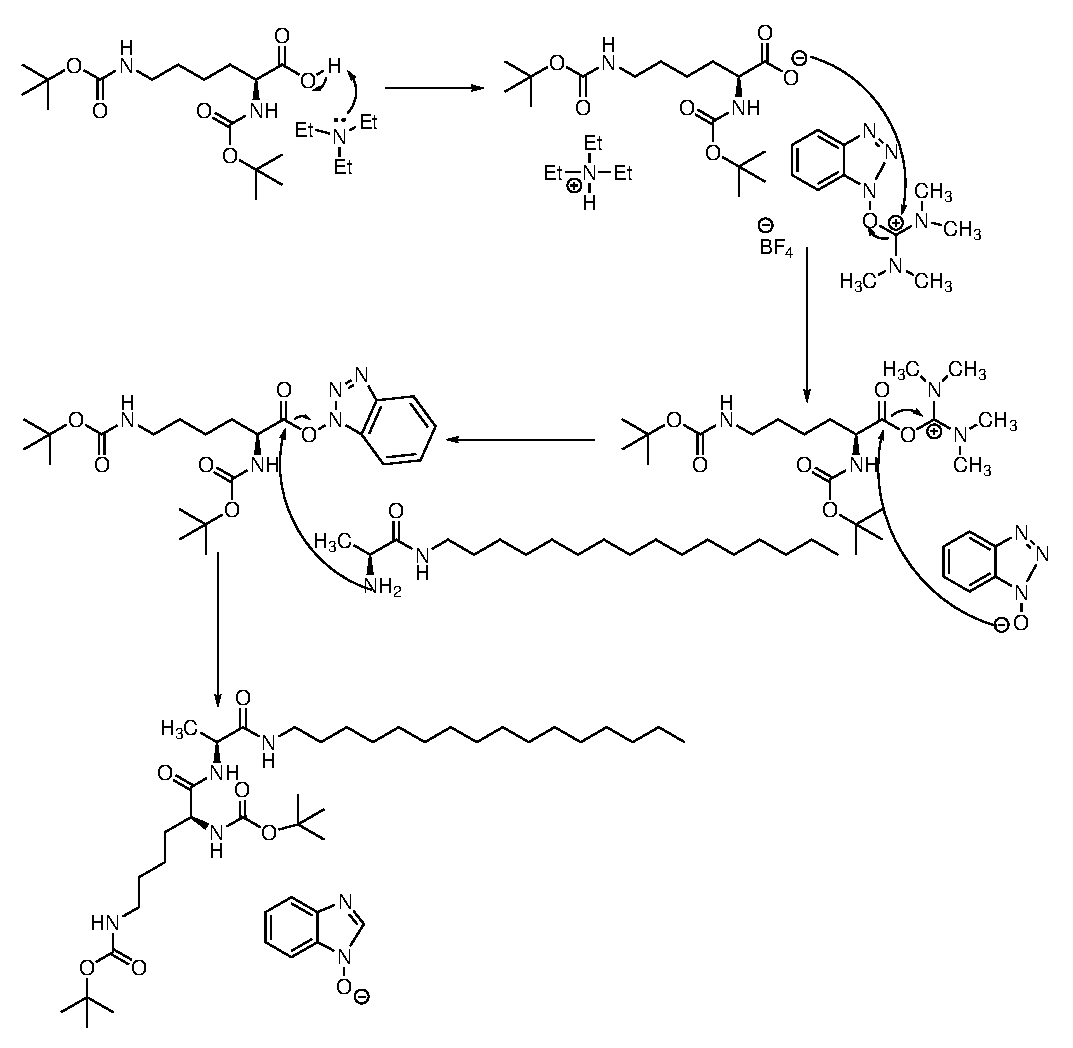
\includegraphics[scale=0.9]{Figures/TBTU_mechanism.eps}
\caption{Mechanism for TBTU mediated peptide coupling}
\label{TBTU mechanism}
\end{figure}
\newpage
\subsection{Adding and Removing Boc-Protecting Groups}
Boc protecting groups are used in this synthesis to generate regioselectivity in the reaction, which then results in only one isomer of product being formed. This has been achieved using Boc anhydride and sodium hydroxide as the base. The mechanism for this is shown in Figure \ref{Boc_protection}. 
\begin{figure}[ht!]
\centering
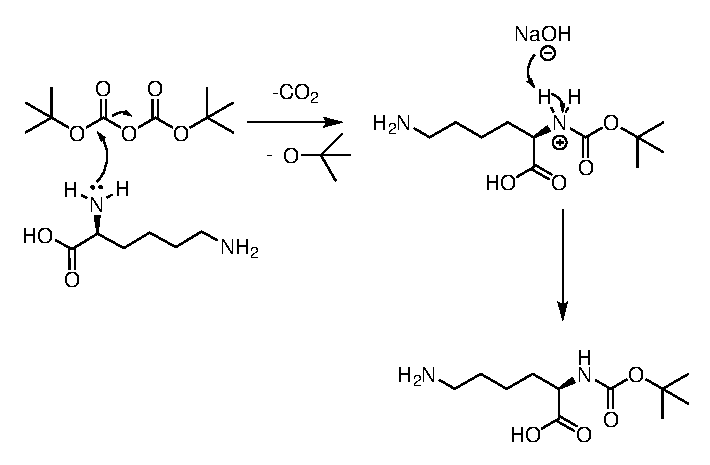
\includegraphics[scale=1]{Figures/Boc_protection.eps}
\caption{Mechanism for Boc protection of L-Ala. Only Boc- protection for one of the NH\textsubscript{2} groups is shown.}
\label{Boc_protection}
\end{figure}

Once the reaction is complete and the desired product has been formed, the protecting groups are no longer useful and need to be removed. There are a variety of ways in which this can be done, but for Boc-deprotection, this reaction is always acid mediated  (Figure \ref{Boc_deprotection}).
\begin{figure}[ht!]
\centering
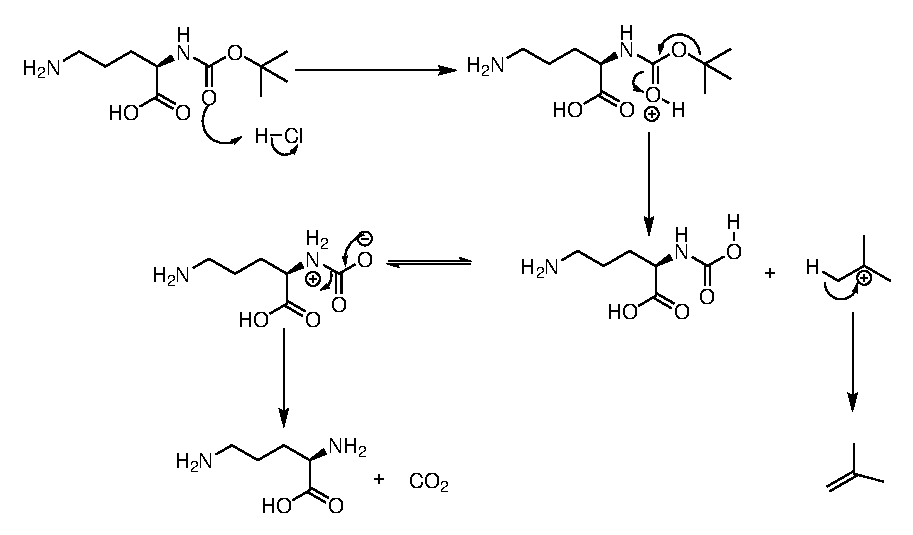
\includegraphics[scale=1]{Figures/Boc_deprotection.eps}
\caption{Mechanism for Boc-deprotection of L-Ala(Boc). Only Boc-deprotection for one NH\textsubscript{2} group is shown.From \cite{Clayden2012OrganicChemistry}} 
\label{Boc_deprotection}
\end{figure}
\newpage
In this work, both dissolving the Boc-protected product in solvent (usually DCM or MeOH), then bubbling HCl gas through the solvent, and dissolving the Boc-protected product into 15 eq. 4 M HCl in dioxane have been used.\footnote{This change is not due to the compounds, but purely due to a limited supply of HCl gas. The author however does have a preference for using 4M HCl in dioxane as this appears to be easier to use.}

Figures \ref{KAT1.16_NMR} and \ref{KAT1.17_NMR} show the effect of dissolving the Boc-protected product 4 M HCl in dioxane, then stirring the solution for one hour. 
Both of these techniques are successful at removing the Boc protecting group - with loss of the \textsuperscript{1}H NMR peak at 1.45 ppm, which corresponds to the Boc group.

\begin{figure}[ht!]
\centering
\includegraphics[scale=0.47]{NMR/KAT1_16.pdf}
\caption{\textsuperscript{1}H NMR C\textsubscript{16}-L-Ala(Boc)}
\label{KAT1.16_NMR}
\end{figure}
\begin{figure}[ht!]
\centering
\includegraphics[scale=0.47]{NMR/KAT1_17.pdf}
\caption{\textsuperscript{1}H NMR of C\textsubscript{16}-L-Ala after removal of Boc-protecting group using 4 M HCl in dioxane}
\label{KAT1.17_NMR}
\end{figure}

\newpage
\subsection{NMR Analysis of Target Compounds}
The four target compounds - C\textsubscript{16}-L-Ala-L-Lys, C\textsubscript{16}-L-Ala-D-Lys, C\textsubscript{16}-D-Ala-L-Lys and C\textsubscript{16}-D-Ala-D-Lys have all been successfully synthesised. These constitute two enantiomeric pairs of binders which have a diastereomeric relationship to each other. The \textsuperscript{1}H NMR spectra are presented in Figures \ref{KAT1.19_NMR} to \ref{KAT1.30_NMR}. 

These NMR spectra are broadly similar to each other; as would be expected. Key proton resonances all appear at equivalent ppm values (Table \ref{NMR_shift}). However, it is clear that the coupling patterns of the CH\textsubscript{2}-N protons are somewhat more complex for the homochiral pair (L,L/D,D) in comparison to the heterochiral pair (L,D/D,L). which is most apparent for the resonances at ca. 3.1 ppm. This reflects the diastereomeric relationship of these two pairs of compounds, leading to differences in coupling, possibly induced by conformational differences between the molecules, leading to subsequent change in torsion angle between coupled protons. 
\newline
\begin{table}[h!]
\centering
\caption{A summary of the differences of chemical shift in \textsuperscript{1}H NMR, between the four target compounds}
\begin{tabular}{l|l|l|l|l}
\textbf{Compound Name} & \textbf{Ala (CH) \textdelta}  & \textbf{Lys (CH) \textdelta} & \textbf{CH\textsubscript{2}-j \textdelta} & \textbf{CH\textsubscript{2}-b \textdelta} \\
\hline
\textbf{C\textsubscript{16}-L-Ala-L-Lys} & 4.31 & 3.91  & 3.12 & 2.97 \\
\textbf{C\textsubscript{16}-D-Ala-D-Lys} & 4.29 & 3.90 & 3.15 & 2.95 \\
\textbf{C\textsubscript{16}-D-Ala-L-Lys} & 4.32 & 3.92 & 3.17 & 2.95 \\
\textbf{C\textsubscript{16}-L-Ala-D-Lys} & 4.32 & 3.92 & 3.17 & 2.97\\
\end{tabular}
\label{NMR_shift}
\end{table}

\newpage
\begin{figure}[ht!]
\centering
\includegraphics[scale=0.47]{NMR/KAT1_19.pdf}
\caption{\textsuperscript{1}H NMR of C\textsubscript{16}-L-Ala-L-Lys}
\label{KAT1.19_NMR}
\end{figure}

\begin{figure}[ht!]
\centering
\includegraphics[scale=0.47]{NMR/KAT1_35.pdf}
\caption{\textsuperscript{1}H NMR of C\textsubscript{16}-D-Ala-D-Lys}
\label{KAT1.35_NMR}
\end{figure}

\begin{figure}[ht!]
\centering
\includegraphics[scale=0.47]{NMR/KAT1_22.pdf}
\caption{\textsuperscript{1}H NMR of C\textsubscript{16}-D-Ala-L-Lys}
\label{KAT1.22_NMR}
\end{figure}

\newpage
\begin{figure}[ht!]
\centering
\includegraphics[scale=0.47]{NMR/KAT1_30.pdf}
\caption{\textsuperscript{1}H NMR of C\textsubscript{16}-L-Ala-D-Lys}
\label{KAT1.30_NMR}
\end{figure}

\begin{table}[h!]
\centering
\caption{A summary of the differences of chemical shift in \textsuperscript{13}C NMR, between the four target compounds}
\begin{tabular}{l|l|l|l|l}
\textbf{Compound Name} & \textbf{Ala (CH) \textdelta}  & \textbf{Lys (CH) \textdelta} & \textbf{CH\textsubscript{2}-NH \textdelta} & \textbf{CH\textsubscript{2}-NH\textsubscript{2} \textdelta} \\
\hline
\textbf{C\textsubscript{16}-L-Ala-L-Lys} & 50.81 & 54.04 & 40.37 & 33.21  \\
\textbf{C\textsubscript{16}-D-Ala-D-Lys} &  50.80 & 54.02 & 40.59 & 33.22 \\
\textbf{C\textsubscript{16}-D-Ala-L-Lys} &  50.90 & 54.35 & 40.44 & 33.22  \\
\textbf{C\textsubscript{16}-L-Ala-D-Lys} &  50.92 & 54.36 & 40.65 & 33.21 \\
\end{tabular}
\label{13CNMR_shift}
\end{table}
\newpage
As with the results obtained from \textsuperscript{1}H NMR, the results from \textsuperscript{13}C NMR are broadly equivalent to each other, with key resonances appearing at equivalent ppm values. The \textsuperscript{13}C NMR spectra are presented in Figures \ref{KAT1.19_13CNMR} to \ref{KAT1.30_13CNMR}. However, in this case, the resonances of the carbon atoms at the chiral centres within these molecules varies much more significantly. This difference in \textsuperscript{13}C NMR highlights the differences between the two diastereotopic pairs of binders that have been synthesised in this work. This further supports the hypothesis posed earlier that the two pairs of molecules adopt differing conformational arrangements in solution. 

\begin{figure}[ht!]
\centering
\includegraphics[scale=0.47]{13CNMR/KAT1_19_13C.pdf}
\caption{\textsuperscript{13}C NMR of C\textsubscript{16}-L-Ala-L-Lys}
\label{KAT1.19_13CNMR}
\end{figure}
\newpage
\begin{figure}[ht!]
\centering
\includegraphics[scale=0.47]{13CNMR/KAT1_35_13C.pdf}
\caption{\textsuperscript{13}C NMR of C\textsubscript{16}-D-Ala-D-Lys}
\label{KAT1.35_13CNMR}
\end{figure}

\begin{figure}[ht!]
\centering
\includegraphics[scale=0.47]{13CNMR/KAT1_22_13C.pdf}
\caption{\textsuperscript{13}C NMR of C\textsubscript{16}-D-Ala-L-Lys}
\label{KAT1.22_13CNMR}
\end{figure}
\newpage
\begin{figure}[ht!]
\centering
\includegraphics[scale=0.47]{13CNMR/KAT1_30_13C.pdf}
\caption{\textsuperscript{13}C NMR of C\textsubscript{16}-L-Ala-D-Lys}
\label{KAT1.30_13CNMR}
\end{figure}

\subsection{Compounds synthesised} 
From the compounds that have been synthesised in this work, several insights have been obtained. 
\begin{enumerate}
\item The protocol for the synthesis of the C\textsubscript{16}-Gly-L/D-Lys as previously published by Chan \textit{et al.} does not necessarily give high yields for the synthesis of this new family of self-assembling heparin binders.
\item Some of these products are hygroscopic, which leads to difficulties in handling.
\item Both bubbling HCl gas through the solvent in which the Boc-protected product has been dissolved, or by dissolving the Boc-protected product in 4M HCl in dioxane will successfully remove the Boc protecting group. 
\item The relationships between these target molecules leads to differences between them, which can be seen in both \textsuperscript{1}H and \textsuperscript{13}C NMR of these target compounds. 
\end{enumerate}

\begin{table}[h!]
\centering
\caption{A summary of the compounds that have been successfully synthesised}
\begin{tabular}{l|l||l|l}
\textbf{Compound name} & \textbf{Yield} & \textbf{Compound name} & \textbf{Yield}\\
\hline
L-Lys(Boc)\textsubscript{2}& 43\% & D-Lys(Boc)\textsubscript{2} & 88\% \\

C\textsubscript{16}-L-Ala(Boc)\textsubscript{2}& 51\% & C\textsubscript{16}-D-Ala(Boc)\textsubscript{2} & 67\% \\

C\textsubscript{16}-L-Ala & 74\% & C\textsubscript{16}-D-Ala &  98\% \\

C\textsubscript{16}-L-Ala-L-Lys(Boc)\textsubscript{2} & 88\% & C\textsubscript{16}-D-Ala-L-Lys(Boc)\textsubscript{2}&  59\% \\

C\textsubscript{16}-L-Ala-L-Lys & 41\% &
C\textsubscript{16}-D-Ala-L-Lys & 82\%\\

C\textsubscript{16}-L-Ala-D-Lys(Boc)\textsubscript{2} & 86\% &
C\textsubscript{16}-D-Ala-D-Lys(Boc)\textsubscript{2}& 91\% \\

C\textsubscript{16}-L-Ala-D-Lys& 81\% & 
C\textsubscript{16}-D-Ala-D-Lys & 95\% \\

\end{tabular}
\label{compounds_synthesised}
\end{table}
\newpage

\section{Assessing Self-Assembly}
Several methods have been used to probe the self-assembly behaviour of the novel binders that have been synthesised in this work. These methods are:
\begin{itemize}
\item Nile Red Assay
\item Dynamic Light Scattering (DLS)
\item Transmission Electron Microscopy (TEM)
\end{itemize}
The theoretical background and results obtained from each of these methods is discussed in detail below.

\subsection{Nile Red Assay}
The aggregation behaviour in solution of these novel heparin binders can be probed by using Nile Red.  Nile Red is a known solvatochromic fluorophore, where a change in polarity of the solvent alters the colour of the solution as well as influencing fluorescence intensity.\textsuperscript{\cite{NileRed-ThermoFisherScientificHttps://www.thermofisher.com/order/catalog/product/N1142}}

Nile Red is (unsurprisingly) red in polar solvents, such as ethanol and undergoes a significant blue-shift in colour when exposed to non-polar solvents. Importantly, it only fluoresces weakly in polar solvents and strongly in non-polar solvents.\textsuperscript{\cite{NileRed-ThermoFisherScientificHttps://www.thermofisher.com/order/catalog/product/N1142}}

These properties of Nile Red have been frequently used within the literature. Plenderleith \textit{et al.} used the colour changing properties of the dye to probe the morphology in water of a highly branched polymer chain at varying temperatures.\textsuperscript{\cite{Plenderleith2014Highly-branchedTemperature}} In polar environments, i.e. in the open coil form of the polymer, the \textlambda\textsubscript{max} of the solution was 660 nm. In the non-polar environment of the globular form, \textlambda\textsubscript{max} fell significantly.
\newline 
Bongiovanni \textit{et al.} exploited both the fluorogenic and solvatochromic properties of the dye to map hydrophobic areas of various biological structures - particularly amyloid aggregates which are already known to play a role in a variety of neurodegenerative disorders including Alzheimers disease.\textsuperscript{\cite{Bongiovanni2016Multi-dimensionalMapping}}
\newline
\begin{figure} [ht!]
\centering
\includegraphics{Nile_Red_Assays/Nile_Red_structure.eps}
\caption{Structure of Nile Red}
\label{Nile_red}
\end{figure}

Nile Red is a known fluorophore, due to the extended conjugation within the molecule (Figure \ref{Nile_red}). Nile Red has been used to assess the self-assembly of surfaces in polar solvents. In the absence of self-assembly, the fluorescence will be weak as the dye experiences the polar solvent environment. However, once self-assembly occurs, the Nile Red partitions into the non-polar, hydrophobic domain often in the centre of the system and fluorescence intensity increases. This behaviour then allows the Critical Aggregation Concentration (CAC) to be assessed. A Nile Red Assay, therefore, monitors the fluorescence of a solution of Nile Red in a polar solvent in the presence of increasing amount of surfactant (in this case, the novel SAMul binders), The concentration at which the fluorescence intensity starts to increase can be taken as an estimation of the CAC value. 

\begin{figure} [ht!]
\centering
\includegraphics[scale=0.45]{Nile_Red_Assays/Nile_Red_Assay_KAT1_19.pdf}
\caption{Fluorescence intensity of Nile Red at 635 nm  in the presence of increasing concentration of C\textsubscript{16}-L-Ala-L-Lys in Tris-HCl buffer.}
\label{NR_KAT1.19}
\end{figure}

\begin{figure} [ht!]
\centering
\includegraphics[scale=0.45]{Nile_Red_Assays/Nile_Red_Assay_KAT1_35.pdf}
\caption{Fluorescence intensity of Nile Red at 635 nm  in the presence of increasing concentration of C\textsubscript{16}-D-Ala-D-Lys in Tris-HCl buffer.}
\label{NR_KAT1.35}
\end{figure}

\begin{figure} [ht!]
\centering
\includegraphics[scale=0.45]{Nile_Red_Assays/Nile_Red_Assay_KAT1_22.pdf}
\caption{Fluorescence intensity of Nile Red at 635 nm  in the presence of increasing concentration of C\textsubscript{16}-D-Ala-L-Lys in Tris-HCl buffer.}
\label{NR_KAT1.22}
\end{figure}

\begin{figure} [ht!]
\centering
\includegraphics[scale=0.45]{Nile_Red_Assays/Nile_Red_Assay_KAT1_30.pdf}
\caption{Fluorescence intensity of Nile Red at 635 nm  in the presence of increasing concentration of C\textsubscript{16}-L-Ala-D-Lys in Tris-HCl buffer.}
\label{NR_KAT1.30}
\end{figure}
\newpage

If the novel heparin binders did not aggregate in Tris HCl, the fluorescence intensity at 635 nm would remain unchanged, despite changing the concentration of binder solution. From Figures \ref{NR_KAT1.19}-\ref{NR_KAT1.22}, it can be seen that this is not the case. Once the concentration of the binder solution reaches a particular concentration, the intensity increases sharply. Therefore, the data set can be split in two; a set where intensity remains almost unchanged, and a data set where it increases sharply.  The point where these two data sets intersect, allows the critical aggregation concentration (CAC) of the binder to be determined. 

The CAC of each novel binder has been determined in this way and displayed in Table \ref{CAC_summary}. The errors are reported as standard deviation and have been obtained by LINEST analysis. 
\newline
\begin{table}[ht!]
\centering
\caption{A summary of the Critical Aggregation Concentrations of each compound.}
\begin{tabular}{l|l}
\textbf{Compound name} &\textbf{CAC /\textmu M}\\
\hline
\textbf{C16-L-Ala-L-Lys} & 50 $\pm$ 3 \\

\textbf{C16-D-Ala-D-Lys} & 44 $\pm$ 3 \\

\textbf{C16-L-Ala-D-Lys} & 166 $\pm$ 3 \\

\textbf{C16-D-Ala-L-Lys} & 155 $\pm$ 3 \\

\end{tabular}
\label{CAC_summary}
\end{table}

These results show that pleasingly, all four novel binders do aggregate in Tris-HCl buffer solution. For C\textsubscript{16}-L-Ala-L-Lys, the CAC was calculated as 50 \textmu M $\pm$ 3
which is unsurprising when compared to the values obtained by Chan and Vieira for C\textsubscript{16}-Gly-L-Lys (33  \textmu M $\pm$ 3) and C16-DAPMA (38.5 \textmu M $\pm$ 0.4)  respectively.\textsuperscript{\cite{Chan2016ChiralBinding,Vieira2017EmergenceHeparin}} The enantiomeric system,  C\textsubscript{16}-D-Ala-D-Lys had, as expected, essentially the same CAC value. However, the diastereomeric pair of enantiomers C\textsubscript{16}-D-Ala-L-Lys, C\textsubscript{16}-L-Ala-D-Lys had a much larger CAC. This was unexpected, but on reviewing the literature was perhaps not surprising. As these results suggest that the two diastereomeric pairs have very different propensities towards self-assembly. 

It has been reported by Bouteiller \textit{et al.}, that changing the stereochemistry of one amide group of a 1,3,5-benzene-tricarboxamide derived from a valine dodecyl ester (Figure \ref{BTA_structure}), leads to a significant change in the shape of the nanoscale assembly.\textsuperscript{\cite{Caumes2016TuningStereochemistry}}

\begin{figure} [ht!]
\centering
\includegraphics{Figures/BTA_structure.eps}
\caption{Left: BTA(S,S,R)-Val.\newline Right: BTA(S,S,S)Val. 
Adapted from \cite{Caumes2016TuningStereochemistry}.}
\label{BTA_structure}
\end{figure}

BTA(S,S,R)-Val self-assembled into long, rod like structures, whilst BTA(S,S,S)-Val only forms dimers. From spectroscopic analysis and Molecular Dynamics calculations, it was noted that the dimeric form of BTA(S,S,S)-Val was very stable due to a large number of both inter- and intramolecular hydrogen bonds, but BTA(S,S,R)-Val was less stable in this form, and at increasing concentration assembled into rod-like structures.

It was then proposed that this difference in behaviour arises from the chiral mismatch in the "arms" of the molecule leading to slightly weaker hydrogen bonds, and enforcing geometrical constraints on the structure.\textsuperscript{\cite{Caumes2016TuningStereochemistry}} 

It should be noted that the difference between the diastereomeric pairs is much greater than that between C\textsubscript{16}-Lys and C\textsubscript{16}-Gly-Lys studied by Chan \textit{et al.}, where there was little change in CAC on insertion of the glycine spacer group.\textsuperscript{\cite{Chan2016ChiralBinding}} This shows that the insertion of a chiral amino acid as the spacer group has a substantial and dramatic effect on the overall assembly event. 

Secondly, the fact a considerably higher concentration is required for aggregation implies the self-assembled micelles if the diastereomeric systems may have significant structural differences. Further characterisation would be necessary to probe this in further detail (see below). 

\subsection{Dynamic Light Scattering}
%Background
In Dynamic Light Scattering (DLS), the sample is irradiated with light, and the light is scattered by the contents of the sample. This backscattered light at 173\textdegree \space is then measured.  The assumption is made that the object which scatters light is spherical, therefore DLS says very little about the shape of the self-assembled nanostructure. 

The intensity distribution shows how much light is scattered by an object of a particular size, this will inherently be a larger amount for larger objects. The volume distribution shows how many objects of a particular size are scattering the incident light. Hence, the volume distribution more clearly shows the contents of the sample, in terms of statistical probability.

Finally, the polydispersity index (PDI) can tell us useful information about the sample. For a perfectly monodisperse solution, the PDI is equal to 1.0. For these samples under test, the PDI is far away from 1 (generally 0.5-0.6), and hence shows the samples do not contain just one type of assembly, but that different types of aggregates are also present. 

DLS measurements were taken of all four novel nanoscale binders at three different concentrations (0.25 mg ml\textsuperscript{-1}, 0.5 mg ml\textsuperscript{-1} and 1 mg ml\textsuperscript{-1}), all giving a concentration of binder well above the CAC, as determined by Nile Red. The DLS measurements at 0.25 mg ml\textsuperscript{-1} and 1.0 mg ml\textsuperscript{-1} are in Appendix \ref{AppendixD}.

Novel binders were dissolved in 10 mM Tris-HCl + 150 mM NaCl solution, before being passed through a 0.45 \textmu M filter to exclude dust particles. All measurements were obtained from 5 runs, and performed in triplicate. It should be noted that the millimolar concentrations required for DLS, are well above the micromolar concentrations required for anion binding described later in this thesis.

\begin{figure} [ht!]
\centering
\includegraphics[scale=0.47]{DLS/KAT1_19_0_5mg_ml-1_size.pdf}
\caption{Intensity distribution of a 0.5 mg ml\textsuperscript{-1} sample of C\textsubscript{16}-L-Ala-L-Lys}
\label{intensity_0.5_KAT1.19}
\end{figure}
\begin{figure} [ht!]
\centering
\includegraphics[scale=0.47]{DLS/KAT1_19_0_5mg_ml-1_volume.pdf}
\caption{Volume distribution of a 0.5 mg ml\textsuperscript{-1} sample of C\textsubscript{16}-L-Ala-L-Lys}
\label{volume_0.5_KAT1.19}
\end{figure}

%KAT1.35 D-Ala-D-Lys
\begin{figure} [ht!]
\centering
\includegraphics[scale=0.47]{DLS/KAT1_35_0_5mg_ml-1_size.pdf}
\caption{Intensity distribution of a 0.5 mg ml\textsuperscript{-1} sample of C\textsubscript{16}-D-Ala-D-Lys}
\label{intensity_0.5_KAT1.35}
\end{figure}
\begin{figure} [ht!]
\centering
\includegraphics[scale=0.47]{DLS/KAT1_35_0_5mg_ml-1_volume.pdf}
\caption{Volume distribution of a 0.5 mg ml\textsuperscript{-1} sample of C\textsubscript{16}-D-Ala-D-Lys}
\label{volume_0.5_KAT1.35}
\end{figure}

%KAT1.22 D-Ala-L-Lys

\begin{figure} [ht!]
\centering
 \includegraphics[scale=0.47]{DLS/KAT1_22_0_5mg_ml-1_size.pdf}
\caption{Intensity distribution of a 0.5 mg ml\textsuperscript{-1} sample of C\textsubscript{16}-D-Ala-L-Lys}
\label{intensity_distribution_KAT1.22_0.5}
\end{figure}
\begin{figure} [ht!]
\centering
\includegraphics[scale=0.47]{DLS/KAT1_22_0_5mg_ml-1_volume.pdf}
\caption{Volume distribution of a 0.5 mg ml\textsuperscript{-1} sample of C\textsubscript{16}-D-Ala-L-Lys}
\label{volume_distribution_KAT1.22_0.5}
\end{figure}

\begin{figure} [ht!]
\centering
\includegraphics[scale=0.47]{DLS/KAT1_30_0_5mg_ml-1_size.pdf}
\caption{Intensity distribution of a 0.5 mg ml\textsuperscript{-1} sample of C\textsubscript{16}-L-Ala-D-Lys}
\label{size_distribution_KAT1.30_0.5}
\end{figure}
\begin{figure} [ht!]
\centering
\includegraphics[scale=0.47]{DLS/KAT1_30_0_5mg_ml-1_volume.pdf}
\caption{Volume distribution of a 0.5 mg ml\textsuperscript{-1} sample of C\textsubscript{16}-L-Ala-D-Lys}
\label{Volume_distribution_KAT1.30_0.5}
\end{figure}
\newpage

In general terms, the intensity distributions show two peaks, one at smaller size (<10 nm) corresponding to micellar objects and another at a significantly larger size (100-500 nm) corresponding to aggregation. 
The volume distribution indicates that the dominant species present are the smaller micellar type assemblies for all four novel binders in this work. Table \ref{DLS_summary} collects together the diameters of these objects as well as the observed zeta potentials. 

\begin{table}[ht!]
\centering
\caption{A summary of the data obtained by DLS for each compound.}
\begin{tabular}{l|l|l|l}
\textbf{Compound name} & \textbf{Concentration / mg ml\textsuperscript{-1}} & \textbf{Z-Average / nm} & \textbf{\textzeta-potential /mV}\\
\hline
\textbf{C\textsubscript{16}-L-Ala-L-Lys} & 0.5 & 45.44 $\pm$ 0.98 & 35.5 $\pm$ 3.3 \\

\textbf{C\textsubscript{16}-D-Ala-D-Lys} & 0.5  & 83.83 $\pm$ 2.16 & 39.2 $\pm$ 2.2\\

\textbf{C\textsubscript{16}-L-Ala-D-Lys} & 0.5 & 150.9 $\pm$ 29.97 & 43.3 $\pm$ 0.6\\

\textbf{C\textsubscript{16}-D-Ala-L-Lys}  & 0.5  &  98.51 $\pm$ 3.78 & 46.8 $\pm$ 0.5\\

\end{tabular}
\label{DLS_summary}
\end{table}

The systems which self-assembled more effectively (C\textsubscript{16}-L-Ala-L-Lys and C\textsubscript{16}-D-Ala-D-Lys) broadly showed more reproducible DLS traces, which supports the hypothesis that they form better-defined aggregates in comparison to those formed by C\textsubscript{16}-D-Ala-L-Lys and C\textsubscript{16}-L-Ala-D-Lys. In all cases,however, micelles (<10 nm) appear to nevertheless be the most dominant form of assembly. It should also be noted that some of these larger aggregates observed by DLS are in part, an artifact of the assay being performed at millimolar concentrations and do not fully reflect the micromolar concentrations described later in this work for anion binding.

\subsection{Zeta Potentials}
%Zeta potentials
\textzeta-potentials of all four novel binders were also obtained by DLS at a concentration of 0.5 mg ml\textsuperscript{-1} using folded capilliary cells (DTS1070). Errors are reported as standard deviations. 
\newline
The \textzeta-potential is a measure of the electrostatic charge/ repulsion between molecules. The greater the value of the \textzeta-potential, the more charged the nanoscale interface.

It can be seen from Table \ref{DLS_summary} that all \textzeta-potentials are positive, reflecting the protonation of the lysine binding group at physiological pH. Also, there is slight variation between them. C\textsubscript{16}-L-Ala-L-Lys and C\textsubscript{16}-D-Ala-D-Lys having very similar \textzeta-potentials to each other (within error) while C\textsubscript{16}-L-Ala-D-Lys and C\textsubscript{16}-D-Ala-L-Lys have higher \textzeta-potentials of ca. 45 mV. If binding were to depend solely on charge density, it might be expected that C\textsubscript{16}-L-Ala-D-Lys and C\textsubscript{16}-D-Ala-L-Lys would perform more effectively.\textsuperscript{\cite{Chan2016ChiralBinding}} 
This increased \textzeta-potential for the C\textsubscript{16}-L-Ala-D-Lys and C\textsubscript{16}-D-Ala-L-Lys pair could explain their propensity towards further aggregation in comparison to C\textsubscript{16}-L-Ala-L-Lys and C\textsubscript{16}-D-Ala-D-Lys, and thus explain why larger aggregates are observed by DLS for the former pair of systems.

\subsection{Transmission Electron Microscopy Analysis}
Transmission Electron Microscopy was carried out with significant help from Meg Stark at the University of York.

Transmission Electron Microscopy (TEM) uses electrons to image objects on the nanoscale.\textsuperscript{\cite{Goodhew2001ElectronAnalysis}} These electrons have a wavelength much shorter than that of visible light, which is particularly useful as it dramatically improves the limit of resolution in comparison to an optical microscope and enables imaging across the entire nanoscale size range.  However, TEM is not without its disadvantages. The high vacuum necessary for this technique can sometimes damage delicate assembled structures and the high electron beam energies can often damage the formvar grid itself, leading to holes within the sample. 

The samples for TEM were first dissolved into Milli-Q water before being placed onto the formvar grid. The nanoscale assemblies were then negatively stained using 1\% uranyl acetate and left to dry for 30 minutes. 
\newline
The binders were imaged at a concentration of (1 mg ml\textsuperscript{-1}/ 2.27 mM). %check this?
The images obtained from this concentration allows us to visualise these novel nanoscale binders (Figure \ref{TEM_2}). The largest objects in the TEM image for C\textsubscript{16}-L-Ala-D-Lys may well be attributed to holes within the formvar grid, rather than larger aggregates.
\newpage
\begin{figure} [h!]
\centering
\includegraphics[scale=0.3]{TEM/bindersonly_TEM.png}
\caption{TEM images of all four novel binders imaged in the absence of a polyanion. 
Top left: C\textsubscript{16}-L-Ala-L-Lys, Top right: C\textsubscript{16}-L-Ala-D-Lys. Bottom left: C\textsubscript{16}-D-Ala-L-Lys, Bottom right: C\textsubscript{16}-D-Ala-D-Lys}
\label{TEM_2}
\end{figure}
The nanoscale assemblies present in these samples are approximately 5 nm $\pm$ 1 in diameter. The micelles appear as lighter coloured circular objects against the dark grey background of the formvar grid, and in each case, in agreement with DLS, it is evident that micelles <10 nm in diameter are being formed. Furthermore, these micelles are evidently stable not only under the drying conditions described earlier, but also under the electron beam.  

Clearly, there is some disagreement between the values obtained via DLS and those from the TEM images above. This arises due to the fact that the nanoscale assemblies are in solution for DLS and hence the hydrodynamic diameter (i.e the nanoscale assembly and shell of solvating water molecules) is measured, whilst TEM requires the samples to be dried before they are imaged and therefore measures only the size of the nanoscale assembly.

\subsection{Circular Dichroism}
The Circular Dichroism analysis of the compounds in this work has been performed by Dr Andrew Leech at the University of York. 

%Background%
Circular Dichroism (CD) relies on plane polarised light, and its absorbance by UV-active components of molecules.  A CD signal only results when the left and right handed components of plane polarised light are absorbed to differing extents by a chiral molecule.\textsuperscript{\cite{Kelly2005HowDichroism}} An absorbance at 220 nm is indicative of the molecule within the sample posessing a peptide bond.  

\begin{figure} [ht!]
\centering
\includegraphics[scale=0.47]{CD/CD-LL_DD.pdf}
\caption{Comparison of C\textsubscript{16}-L-Ala-L-Lys and C\textsubscript{16}-D-Ala-D-Lys binders by Circular Dichroism}
\label{CD-LL_DD}
\end{figure}

\begin{figure} [ht!]
\centering
\includegraphics[scale=0.47]{CD/CD-LD_DL.pdf}
\caption{Comparison of C\textsubscript{16}-L-Ala-D-Lys and C\textsubscript{16}-D-Ala-L-Lys binders by Circular Dichroism}
\label{CD-LD_DL}
\end{figure}

%Discussion%
Figures \ref{CD-LL_DD} and \ref{CD-LD_DL} show that two enantiomeric pairs of molecules have successfully been synthesised as the CD spectra show the molecules broadly absorb light in an equal, but opposite fashion. 
\newline
It can also be said that there are significant differences between the diastereomeric pairs e.g. C\textsubscript{16}-L-Ala-L-Lys and C\textsubscript{16}-L-Ala-D-Lys, in terms of both absolute ellipticity and line shape. These differences in CD support the hypothesis posed earlier, on analysis of \textsuperscript{1}H NMR, that these diastereomeric pairs fold themselves in very different ways and help explain why their propensity towards self-assembly differs. 
\newline
However, these CD spectra cannot be used alone to make any suggestions about the way these molecules choose to fold within solution.  

\newpage
\section{Polyanion Binding Studies}
The ability of these systems to bind biological polyanions was then explored. Of particular interest was the determination whether differences in propensity towards self-assembly would also be translated into differences in polyanion binding. 

\subsection{Ethidium Bromide Displacement Assay}
%Background%
Ethidium bromide (EthBr) is an intercalating agent commonly used in molecular biology to stain nucleic acids for visualisation in gel electrophoresis.The central structure of the molecule is a phenanthridine group, which also appears in several other intercalating dyes.\textsuperscript{\cite{EthidiumbromideBioReagent-Sigma-AldrichHttp://www.sigmaaldrich.com/catalog/product/sigma/e7637}} It is this fused ring system that gives EthBr the property that is being exploited in this case. \newline
\begin{figure} [h!]
\centering
\includegraphics{Ethidium_Bromide/EtBr_structure.eps}
\caption{Structure of Ethidium Bromide}
\label{EthBr_structure}
\textsuperscript{\cite{EthidiumbromideBioReagent-Sigma-AldrichHttp://www.sigmaaldrich.com/catalog/product/sigma/e7637}} \end{figure}

For exactly the same reasons as Nile Red, EthBr is also a fluorophore. On binding to DNA, EthBr fluoresces strongly, with \textlambda\textsubscript{max} at 595 nm. This is believed to occur as binding to DNA forces the ethidium bromide to shed bound water molecules, which are known to be successful at quenching fluorescence.\textsuperscript{\cite{Olmsted1977MechanismAcids}}  It is this fluorescence that can be monitored as a competing binder is introduced in solution. If this new binder binds DNA more strongly than EthBr, then EthBr is displaced, and fluorescence intensity decreases. However, some believe that this does not necessarily show the displacement of EthBr by another ligand, but instead suggests the formation of a ternary complex.\textsuperscript{\cite{Banerjee2013FluorescenceDNA}} Nevertheless, this is still an effective comparative method of assaying DNA binders. 

A solution of DNA and EthBr in Tris-HCl buffer is made and the novel binder is titrated into it, with the quenching of fluorescence (and hence the displacement of EthBr) being monitored. This allows quantification of the DNA binding ability of each novel binder, and is particularly useful for comparing similar molecules under identical assay conditions. 

\begin{figure} [ht!]
\centering
\includegraphics[scale=0.47]{Ethidium_Bromide/homochiral_pair_EthBr.pdf}
\caption{Comparison of C\textsubscript{16}-L-Ala-L-Lys and C\textsubscript{16}-D-Ala-D-Lys in EthBr assay}
\label{Etbr_homochiral}
\end{figure}
\begin{figure} [ht!]
\centering
\includegraphics[scale=0.47]{Ethidium_Bromide/heterochiral_pair_EthBr.pdf}
\caption{Comparison of C\textsubscript{16}-L-Ala-D-Lys and C\textsubscript{16}-D-Ala-L-Lys binders in EthBr assay}
\label{Etbr_heterochiral}
\end{figure}
\newpage

Ethidium Bromide displacement assays were performed in triplicate and errors are reported as standard deviations.  From these displacement assays (Table \ref{EtBr_summary}), it is possible to calculate EC\textsubscript{50} and CE\textsubscript{50} values. EC\textsubscript{50} is the effective concentration of binder necessary to displace 50\% of the dye, whilst CE\textsubscript{50}  is the charge excess of the binder when 50\% of the dye has been displaced.

\begin{table}[ht!]
\centering
\caption{A summary of the data obtained from Ethidium Bromide displacement assays.}
\begin{tabular}{l|l|l}
\textbf{Compound name} & \textbf{EC\textsubscript{50} (\textmu M)} & \textbf{CE\textsubscript{50}}\\
\hline
\textbf{C\textsubscript{16}-L-Ala-L-Lys} & 15.61 $\pm$ 2.14  & 7.8 $\pm$ 1.06  \\

\textbf{C\textsubscript{16}-D-Ala-D-Lys} & 9.47 $\pm$ 1.27 & 2.76 $\pm$ 0.36  \\

\textbf{C\textsubscript{16}-D-Ala-L-Lys} &  18.75 $\pm$ 1.15  & 9.37 $\pm$ 0.55\\

\textbf{C\textsubscript{16}-L-Ala-D-Lys} & 6.08 $\pm$ 0.98 & 3.05 $\pm$ 0.48 \\

\end{tabular}
\label{EtBr_summary}
\end{table}
%Discussion%

The results show that all four novel nanostructures successfully displace Ethidium Bromide and bind to DNA at micromolar concentrations. The effective concentrations necessary to bind DNA are all substantially lower than those reported for CAC by the Nile Red assays performed previously. This shows that the presence of DNA may assist self-assembly of the cationic compounds. It could be hypothesised that the negatively charged phosphate groups and the positively charged lysine groups in the novel binders have electrostatic interactions between them, and these interactions that locates the binder close to the DNA. This then leads to a higher concentration of the novel binder around the DNA strands, encouraging self-assembly of the micelles and hence improving binding. 

The lower the value of CE\textsubscript{50} the better the nanoscale interface is at binding DNA and displacing EthBr.  It can clearly be seen that there is a very dramatic preference for D-Lys over L-Lys at the binding interface, with the CE\textsubscript{50} values for C\textsubscript{16}-D-Ala-D-Lys and C\textsubscript{16}-L-Ala-D-Lys being 2.76 $\pm$ 0.36 and 3.05 $\pm$ 0.48 compared to 7.8 $\pm$ 1.06 and 9.37 $\pm$ 0.55. These differences are well beyond the established error range, and hence are considered to be significant. It is remarkable that the enantiomeric systems are so different to one another. Clearly, C\textsubscript{16}-D-Ala-D-Lys is a much better DNA binder than C\textsubscript{16}-L-Ala-L-Lys, despite the fact they both self-assemble in identical ways. The same argument can be made for the C\textsubscript{16}-L-Ala-D-Lys and C\textsubscript{16}-D-Ala-L-Lys pair of compounds. This clearly indicates that the chirality of the lysine is in full control of the binding interface between these systems and DNA. As such, it can confidently be asserted that lysine chirality controls DNA binding affinity, and that both the chirality of the spacer group and propensity towards self-assembly having very limited impact. 

\subsection{Mallard Blue Assay}
%Background%
Mallard Blue (MalB) is a arginine-functionalised thionine dye developed by Bromfield \textit{et al.}, and it is used here in a competition assay to quantify heparin binding.\textsuperscript{\cite{Bromfield2013MallardMedia}} It was noted that several promising novel heparin sensors had been reported in the literature, but they all arose through complex, multi-step synthesis which made them difficult to prepare. It had been hoped that a commerically available thionine dye could be used as a sensor to quantify heparin levels, but no suitable candidate was forthcoming.\textsuperscript{\cite{Bromfield2014MultivalentSensing}} 
\newline

\begin{figure} [h!]
\centering
\includegraphics{Mallard_Blue/Mallard_blue.eps}
\caption{Structure of the novel dye Mallard Blue (MalB)}
\label{Mallard_Blue}
\end{figure}
Instead, Bromfield and coworkers chose to design a novel heparin binder (Figure \ref{Mallard_Blue}).  
The thionine core was chosen due to its fluorogenic \& chromogenic properties, which would then allow the heparin binding ability to be quantified.  The idea to functionalise this thionine core with arginine groups came from the observation that protamine sulfate (which is heavily decorated with arginine groups) functions in human serum and it was hoped that appending these to the thionine core would give the new molecule the ability to bind heparin in human serum and this binding to be unaffected by other biologically relevant anions.\textsuperscript{\cite{Bromfield2014MultivalentSensing}} This was shown to be true, and MalB not only binds heparin in competitive media, the UV-Vis absorption is not peturbed by the presence of other, structurally similar glycosoaminoglycans, but it also has a facile two-step synthesis, which clearly gives this dye advantages over those previously reported.\textsuperscript{\cite{Bromfield2014MultivalentSensing, Bromfield2013ADendrimers.}} 

%how does the Assay work?
Like the EthBr assay, Mallard blue is also a displacement assay and works as follows; the cuvette is charged with heparin sulfate and Mallard Blue. A stock solution of binder is then titrated into this cuvette and the Mallard Blue is displaced by the introduction of the novel binder. This displacement of MalB causes both \textlambda \textsubscript{max} to shift to longer wavelength, and an increase in the absorbance at 615 nm, as MalB functions as a "switch off" sensor for heparin.  From this change in the UV absorbance of the solution, EC\textsubscript{50}, CE\textsubscript{50} and the mass of binder necessary to neutralise a given dose of heparin sulfate can all be obtained. The results are normalised against a cuvette containing Mallard Blue in buffer, and a cuvette containing both MalB and heparin.
As a consequence of all licensed heparin preparations in the EU being of porcine origin, all of the heparin used in this displacement assay is also of porcine origin.\textsuperscript{\cite{Mulloy2015PharmacologyDrugs}}
\newpage
\begin{figure} [h!]
\centering
\includegraphics[scale=0.42]{Mallard_Blue/Homochiral_pair_-_MalB.pdf}
\caption{Binding Assay for C\textsubscript{16}-L-Ala-L-Lys and C\textsubscript{16}-D-Ala-D-Lys}
\label{homochiral_pair}
\end{figure}
\begin{figure} [h!]
\centering
\includegraphics[scale=0.42]{Mallard_Blue/Heterochiral_pair_-_MalB.pdf}
\caption{Binding Assay for C\textsubscript{16}-L-Ala-D-Lys and C\textsubscript{16}-D-Ala-L-Lys}
\label{heterochiral_pair}
\end{figure}
\newpage
Further normalisation has been applied to the results to account for the turbidity of the samples at higher binding concentrations, which resulted in the corrected absorbance rising above 1.0. (Figures \ref{homochiral_pair} \& \ref{heterochiral_pair}).

Firstly, it can be seen that all four novel heparin binders give a sigmoidal line shape in the Mallard Blue assay. At low concentrations of binder, there is very little change in the absorbance at 615 nm, as little MalB is displaced. Once a particular concentration of novel binder is reached, the absorbance at 615 nm increases sharply, this behaviour implies that self-assembly of the novel nanoscale binders is necessary before heparin binding and subsequent MalB displacement becomes possible. This is somewhat different to what is observed in the EthBr assays.

Table \ref{MalB_summary} summarises the values of CE\textsubscript{50}, EC\textsubscript{50}, and the mass necessary for each of the 4 novel binders to neutralise a given dose of heparin. Errors are reported as standard deviations. 
\begin{table}[ht!]
\centering
\caption{A summary of the data obtained from Mallard Blue displacement assay for the novel binders in this work}
\begin{tabular}{l|l|l|l}
\textbf{Compound name} & \textbf{CE\textsubscript{50}} &\textbf{EC\textsubscript{50} (\textmu M)} & \textbf{Dose /mg 100 IU\textsuperscript{-1}} \\
\hline
\textbf{C\textsubscript{16}-L-Ala-L-Lys} &  2.32 $\pm$  0.08 & 125.5  $\pm$ 4.5  &  1.60 $\pm$ 0.05   \\
\textbf{C\textsubscript{16}-D-Ala-D-Lys} &  1.84 $\pm$  0.36 & 110.3 $\pm$ 2.20 &  1.41 $\pm$ 0.02 \\

\textbf{C\textsubscript{16}-D-Ala-L-Lys} & 2.69 $\pm$ 0.22 &  145.2 $\pm$ 12.0 & 1.85 $\pm$ 0.15 \\

\textbf{C\textsubscript{16}-L-Ala-D-Lys} & 2.47 $\pm$ 0.12  & 134  $\pm$ 6.50  & 1.71 $\pm$ 0.08 \\

\textbf{Protamine Sulfate}\textsuperscript{\cite{Bromfield2014NanoscaleMedia}} & 0.52 $\pm$ 0.05 &  2.34 $\pm$ 0.23 & 0.32$\pm$ 0.02 \\

\end{tabular}
\label{MalB_summary}
\end{table}

The CE\textsubscript{50} values obtained from the MalB assay (Table \ref{MalB_summary}) show that heparin binding behaves very differently to DNA binding. Broadly speaking, the binding of C\textsubscript{16}-L-Ala-L-Lys and C\textsubscript{16}-D-Ala-D-similar. This suggests that the chirality of the lysine binding group does not drive the recognition event in this case. For C\textsubscript{16}-L-Ala-D-Lys and C\textsubscript{16}-D-Ala-L-Lys, the former is somewhat better at binding heparin sulfate and suggests that the chirality of the lysine group has some influence in this case.  

It can also be seen that the homochiral pair of binders posess a higher affinity towards binding heparin than their heterochiral counterparts, that have higher CE\textsubscript{50} values. This reflects the similarities in self-assembly behaviour previously shown by Nile Red assays. It could be hypothesised that there is some sort of synergistic effect taking place, where the enhanced propensity towards self-assembly of C\textsubscript{16}-L-Ala-L-Lys and C\textsubscript{16}-D-Ala-D-Lys compared to C\textsubscript{16}-L-Ala-D-Lys and C\textsubscript{16}-D-Ala-L-Lys, enhances heparin binding. This would also agree with the sigmoidal line shape that is observed and that some degree of self-assembly is a pre-requisite for heparin binding. 

It is clear that the EC\textsubscript{50} values are very different to the CAC's reported by the Nile Red assay. This implies that the binders under test here behave differently when presented with heparin. 
The CACs reported by Nile Red for the C\textsubscript{16}-L-Ala-L-Lys and C\textsubscript{16}-D-Ala-D-Lys pair were 50 $\pm$ 3 and 44 $\pm$ 3, whilst the EC\textsubscript{50} vales reported here are 125 $\pm$ 2 and 110 $\pm$ 2 respectively. This indicates that self-assembly is clearly necessary for effective multivalent binding. Whilst the results obtained here show that the C\textsubscript{16}-D-Ala-L-Lys and C\textsubscript{16}-L-Ala-D-Lys pair rely on heparin to some extent to help encourage self-assembly, as the EC\textsubscript{50} values here are lower than the CACs obtained by Nile Red. This increased ability to self-assemble is likely to occur due to the electrostatic interactions between the negatively charged sulfate groups of heparin, and the positively charged lysine residues of the novel binders. 
Smith and co-workers have shown by several previous studies that both charge density and flexibility of the host play a vital role in  the binding of heparin sulfate to protamine.\textsuperscript{\cite{Bromfield2013HeparinApplications, Bromfield2013ADendrimers.,Chan2016ChiralBinding, Bromfield2014Shape-PersistentBinding,Vieira2017EmergenceHeparin,Fechner2016ElectrostaticBinding}} 

\begin{table}[ht!]
\centering
\caption{A summary of the data obtained by Chan \textit{et al.} for their novel binders. From \cite{Chan2016ChiralBinding}.}
\begin{tabular}{l|l|l}
\textbf{Compound name} & \textbf{CE\textsubscript{50}} &\textbf{EC\textsubscript{50} (\textmu M)}  \\
\hline
\textbf{C\textsubscript{16}-L-Lys} &  1.8 $\pm$ 0.1  &  100 $\pm$ 3  \\
\textbf{C\textsubscript{16}-D-Lys} &  1.8  $\pm$ 0.1  &  100$\pm$ 3  \\
\textbf{C\textsubscript{16}-Gly-L-Lys} & 3.3 $\pm$ 0.3 & 180  $\pm$ 17 \\
\textbf{C\textsubscript{16}-Gly-D-Lys} & 2.3 $\pm$ 0.1 & 122  $\pm$ 2\\
\end{tabular}
\label{Chan_MalB}
\end{table}
It should be noted that the enantioselectivity of heparin binding previously reported by Chan and Smith (Table \ref{Chan_MalB}), is still observed here, specifically for C\textsubscript{16}-L-Ala-D-Lys and C\textsubscript{16}-D-Ala-L-Lys despite changing the amino acid spacer group from the achiral glycine to the chiral amino acid lysine. However, the enantioselectivity is not observed for the diastereometic C\textsubscript{16}-L-Ala-L-Lys/ C\textsubscript{16}-D-Ala-D-Lys pair. This suggests that the precise mode of self-assembly (and hence ligand display) plays a vital role in determining whether enantioselective binding is observed at the nanoscale interface. 
 
All 4 of the novel binders reported in Table \ref{MalB_summary} bind heparin sulfate in Tris-HCl buffer. However, on comparison to the data obtained by Bromfield et al. for the binding affinity of protamine sulfate to heparin, none of the four binders synthesised in this work required a lower dose to neutralise the effect of 100 IU of heparin, than protamine sulfate did in these particular conditions.\textsuperscript{\cite{Bromfield2014NanoscaleMedia}} This shows that, unfortunately, these novel heparin binders are not more effective in Tris-HCl buffer than protamine sulfate. 

Finally, if the results for both the Ethidium Bromide and Mallard Blue assays are considered together, it can be shown that the flexibility of the host also plays a vital role in the binding of these novel binders to a given biological polyanion. The lack of flexibility in the structure of DNA leads to much greater stereoselectivity. It has been noted by Fechner, Albanyan \textit{et al.}, that heparin sulfate is a “adaptive” polyanion, i.e. it changes itself in response to the SAMul binding surface it is presented with, whilst the opposite is true of DNA and it will attempt to organise the SAMul interface, for this reason it can be suggested that rigid DNA, with its well-defined display of phosphate anions has a much greater enantio-preference programmed into it.\textsuperscript{\cite{Fechner2016ElectrostaticBinding}}

It is known from work by Vieira \textit{et al.} that a large value for the \textzeta-potential does not necessarily indicate that this is the best heparin binder.\textsuperscript{\cite{Vieira2017EmergenceHeparin}} C\textsubscript{16}-D-Ala-L-Lys, is highly charged according to its \textzeta-potential, but a poor heparin binder as determined by the MalB assay. However, it was seen by Albanyan \textit{et al.} that the greater the \textzeta-potential for a given molecule, the greater the driving force for self-assembly.\textsuperscript{\cite{Albanyan2017Self-AssembledLigands}}

\subsection{TEM Analysis of Polyanion Binding}
Since both Mallard Blue and Ethidium Bromide displacement assays have been performed on these novel binders, it makes sense to also image these binders in the presence of both DNA and heparin sulfate. 

These images at x49000 magnification show how the presence of DNA encourages the nanoscale micelles to self-assemble into larger aggregates (Figure \ref{TEM_DNA1}).  The presence of unbound micelles is due to the high concentration of binder within these samples. 
\newline
Using the information obtained from the analysis presented previously, it is known that the presence of DNA encourages the binders to undergo self assembly at an effective concentration much lower than the CAC, and that this concentration of binder solution is known to encourage further self-assembly into larger aggregates. 
Therefore, it can be said that the binders must form these large aggregates that can be seen on the TEM images on binding DNA. A further set of images at x120k magnification show these larger aggregates even more clearly (Figure \ref{TEM_DNA2}). 

Excitingly, all 4 binders form aggregates much smaller than 150 nm, Ghosh et al. determined that endocytosis is limited to objects under 150 nm in size. This suggests these Ala-Lys systems could be useful DNA transfection agents.\textsuperscript{\cite{Ghosh2008EfficientNanoparticles}}
\newpage
\begin{figure} [h!]
\centering
\includegraphics[scale=0.3]{TEM/binders_DNA_49000.png}
\caption{TEM images of all four novel binders imaged in the presence of DNA. x49000 magnification
Top left: C\textsubscript{16}-L-Ala-L-Lys, Top right: C\textsubscript{16}-L-Ala-D-Lys. Bottom left: C\textsubscript{16}-D-Ala-L-Lys, Bottom right: C\textsubscript{16}-D-Ala-D-Lys}
\label{TEM_DNA1}
\end{figure}

\newpage
\begin{figure} [h!]
\centering
\includegraphics[scale=0.3]{TEM/binders_DNA_120k.png}
\caption{TEM images of all four novel binders imaged in the presence of DNA. x120k magnification
Top left: C\textsubscript{16}-L-Ala-L-Lys, Top right: C\textsubscript{16}-L-Ala-D-Lys. Bottom left: C\textsubscript{16}-D-Ala-L-Lys, Bottom right: C\textsubscript{16}-D-Ala-D-Lys}
\label{TEM_DNA2}
\end{figure}

\newpage
%Binding Heparin sulfate
It is known from previous work that molecules which self-assemble into spherical morphologies are the best heparin binders.\textsuperscript{\cite{Barnard2012Self-AssembledBinding}} From the images in Figure \ref{TEM_heparin1} it can be seen that all 4 novel binders do form spherical aggregates, some of which clearly then undergo further self-assembly to form larger, non-spherical assemblies. This certainly mirrors the results obtained from the MalB assay, i.e. that all 4 novel binders bind heparin at micromolar concentrations. 

To some extent, the "beads on a string" phenomenon reported previously by Campo-Rodrigo \textit{et al.} for their self-assembling dendrons capable of binding heparin can be seen in the TEM images presented in Figures \ref{TEM_heparin1} \& \ref{TEM_heparin2}.\textsuperscript{\cite{Rodrigo2011Self-AssemblingBinding}} The phenomenon had been seen repeatedly and reported several years earlier for the binding of spherical cationic systems to DNA, and this hierarchical binding has been fully characterised by Vieira \textit{et al.}, where it is viewed as being anion-induced close packing of cationic spheres.\textsuperscript{\cite{Vieira2017EmergenceHeparin,Wong2007AnLength}}. This phenomenon helps explain why the results presented previously for anion binding in Tables \ref{EtBr_summary} \& \ref{MalB_summary} state that more than one positive charge on the binder is necessary to bind one negative charge from either heparin sulfate or DNA. The TEM images presented in this section show that not all of the positive charges on these nanoscale assemblies are capable of binding directly to the biological polyanion that they have been presented with. 

In all cases, the TEM images look reasonably similar, suggesting that differences in DNA and heparin binding cannot simply be attributed to different morphologies of the self-assembled nanosystems.

\newpage
\begin{figure} [h!]
\centering
\includegraphics[scale=0.3]{TEM/binders_heparin_49000.png}
\caption{TEM images of all four novel binders imaged in the presence of heparin sulfate. x49000 magnification
Top left: C\textsubscript{16}-L-Ala-L-Lys, Top right: C\textsubscript{16}-L-Ala-D-Lys. Bottom left: C\textsubscript{16}-D-Ala-L-Lys, Bottom right: C\textsubscript{16}-D-Ala-D-Lys}
\label{TEM_heparin1}
\end{figure}

\newpage
\begin{figure} [h!]
\centering
\includegraphics[scale=0.3]{TEM/binders_heparin_120k.png}
\caption{TEM images of all four novel binders imaged in the presence of heparin sulfate. x120k magnification
Top left: C\textsubscript{16}-L-Ala-L-Lys, Top right: C\textsubscript{16}-L-Ala-D-Lys. Bottom left: C\textsubscript{16}-D-Ala-L-Lys, Bottom right: C\textsubscript{16}-D-Ala-D-Lys}
\label{TEM_heparin2}
\end{figure}
\newpage



\chapter{Summary and Conclusions} % Main chapter title
\label{Chapter3} %

\section{Synthesis of novel nanostructures}
Two enantiomeric pairs of target compounds have been successfully synthesised via a synthetic method  developed in this work, and their identity confirmed by \textsuperscript{1}H, \textsuperscript{13}C and DEPT-135 NMR, Mass Spectrometry and Infrared Spectroscopy.  It has been noted that modifying the amino acid spacer group has a substantial effect on the solubility of some intermediate products. This was unexpected, but from previous work, it is not surprising that a small change in the structure of these types of molecules leads to a large change in their behaviour.\textsuperscript{\cite{Vieira2017EmergenceHeparin,Albanyan2017Self-AssembledLigands}}  

There are a variety of possible ways to remove the Boc-protecting groups from these products. Both dissolving the Boc-protected product in DCM before bubbling HCl gas through the solution and dissolving the product in 4M HCl in dioxane have been used and both successfully remove the protecting group, as shown by \textsuperscript{1}H NMR. 

\textsuperscript{1}H NMR has also been used to show that there are subtle differences between the four novel heparin binders in this work. Key proton resonances all appear at equivalent ppm values. However, the coupling patterns of the CH\textsubscript{2}-N protons differ between the two diastereotopic pairs of compounds, allowing them to be distinguished. Also proving that the chirality of the amino acid building blocks does not get scrambled during synthesis, and suggests that the diastereomers may have different conformational preferences. 

\section{Assessing Self-Assembly}
\subsection{Nile Red Assay}
The Nile Red assays show that all four novel heparin binders successfully aggregate in solution, and the calculated CAC values for the C\textsubscript{16}-L-Ala-L-Lys, C\textsubscript{16}-D-Ala-D-Lys pair of molecules are similar to those obtained by Vieira and Chan for C\textsubscript{16}-DAPMA and C\textsubscript{16}-Gly-L-Lys respectively.\textsuperscript{\cite{Vieira2017EmergenceHeparin,Chan2016ChiralBinding}}
It also shows that the insertion of the chiral amino acid alanine does have an effect on the properties of the overall nanoscale assembly, as the CAC value increases significantly from 45 \textmu M for C\textsubscript{16}-L-Ala-L-Lys/C\textsubscript{16}-D-Ala-D-Lys to 160 \textmu M for the diastereomeric pair C\textsubscript{16}-D-Ala-L-Lys and C\textsubscript{16}-L-Lys-D-Ala. This dramatic increase in CAC value was not observed by Chan \textit{et al.} on the insertion of the achiral amino acid glysine into C\textsubscript{16}-Lys, but changing chirality leading to significant changes in behaviour has been reported previously by Boutellier \textit{et al.} for a 1,3,5-benzene-tricarboxamide system.\textsuperscript{\cite{Chan2016ChiralBinding,Caumes2016TuningStereochemistry}} It suggests that the conformational change observed by \textsuperscript{1}H NMR significantly impacts on the ability of these compounds to self-assemble. It is hypothesised that the head group becomes more sterically hindered and less able to self-assemble effectively. 

\subsection{Dynamic Light Scattering}
DLS can be used to obtain a large variety of information about a sample, however, one of the main assumptions made by DLS is that the objects which scatter light are spherical. Hence this analytical method can say very little about the shape of the self-assembled heparin binders in solution. Despite this, the polydispersity index (PDI), Intensity and Volume distributions hold useful information. 

The PDI of these samples is between 0.5 and 0.6, indicating that these samples are not monodisperse (PDI = 1.0) and that a range of different sized objects must be present within the sample. This implies the presence of aggregates within the solution. 

In general terms, the intensity distributions show two distinct peaks; one at smaller size (<10 nm) that corresponds to the micellar objects, and a second at a substantially larger size (100-500 nm), indicating the presence of aggregates within the sample. The volume distribution indicates that the dominant species in each sample are these smaller micellar-type assemblies.  

It can also be seen that the systems which self-assemble more effectively also broadly appear to posses more reproducible DLS traces, which helps support the hypothesis that they form better defined aggregates in comparison to those formed by C\textsubscript{16}-D-Ala-L-Lys and C\textsubscript{16}-L-Ala-D-Lys. It should also be noted that some of these larger aggregates that have been observed are an artifact of the assay being performed at micromolar concentrations - this higher concentration  encourages further self-assembly. 

\subsection{Zeta potentials}
The zeta potentials obtained for all four target compounds are positive. This shows that the lysine binding groups on the nanoscale interface are protonated at physiological pH. 
\newline
C\textsubscript{16}-L-Ala-L-Lys and C\textsubscript{16}-D-Ala-D-Lys having very similar \textzeta-potentials to each other (within error) while C\textsubscript{16}-L-Ala-D-Lys and C\textsubscript{16}-D-Ala-L-Lys have higher \textzeta-potentials of ca. 45 mV. If binding were to depend solely on charge density, it might be expected that C\textsubscript{16}-L-Ala-D-Lys and C\textsubscript{16}-D-Ala-L-Lys would perform more effectively.\textsuperscript{\cite{Chan2016ChiralBinding}} 
\newline
This increased \textzeta -potential for the C\textsubscript{16}-L-Ala-D-Lys and C\textsubscript{16}-D-Ala-L-Lys pair could explain their propensity towards further aggregation in comparison to C\textsubscript{16}-L-Ala-L-Lys and C\textsubscript{16}-D-Ala-D-Lys, and thus explain why larger aggregates are observed by DLS for the former pair of systems.

\subsection{Transmission Electron Microscopy Analysis}
Transmission Electron Microscopy was used to image the nanoscale binders alone, and in the presence of both biological polyanions of interest in this work. It can be shown by TEM that the nanoscale binders undergo self-assembly, and the micelles have a diameter of 5 $\pm$ 1 nm. This is smaller than the diameter observed via DLS, this occurs because of the differing conditions in which the micelles are sized. DLS measures the micelles in solution and therefore determines hydrodynamic diameter, whilst TEM samples are dried and hence only the nanoscale assembly itself is observed. 

\subsection{Circular Dichroism}
Circular Dichroism shows that the four target compounds synthesised in this work comprise of two enantiomeric pairs of molecules, which absorb plane polarised light in a broadly equal and opposite fashion. 
\newline
It has also been noted that there are significant differences between the CD spectra obtained for the diastereomeric pairs e.g. C\textsubscript{16}-L-Ala-L-Lys and C\textsubscript{16}-L-Ala-D-Lys, in terms of both absolute ellipticity and line shape. These differences in CD help support the hypothesis that these diastereomeric pairs fold themselves in very different ways and help explain why they possess differing propensities towards self-assembly. 
\section{Polyanion Binding Studies}
\subsection{Ethidium Bromide Displacement Assay}
The results from the Ethidium Bromide displacement assay show that all four novel nanostructures do bind DNA and successfully displace EthBr at micromolar concentrations. Again, this is much lower than the CAC determined by Nile Red and implies that the presence of DNA has an effect on binding the biological polyanion. CE\textsubscript{50} values show a dramatic preference for D-Lys as the binding group over L-Lys. This suggests that the binding interface with DNA is dominated by the precise interaction with the lysine binding group, which is determined by chirality. The chirality of the alanine spacer group, and the diastereomeric nature of the self-assembled systems appear to have no effect on the recognition interface. 

\subsection{Mallard Blue Assay}
Mallard Blue assays have shown that if the target compounds are unable to self-assemble, then their heparin binding ability is "switched off".  It can be stated that self-assembly  of these compounds is necessary before heparin binding and MalB displacement is possible. 

CE\textsubscript{50} values show that the C\textsubscript{16}-L-Ala-L-Lys and C\textsubscript{16}-D-Ala-D-Lys pair behave similarly to each other, and so too do C\textsubscript{16}-L-Ala-D-Lys and C\textsubscript{16}-D-Ala-L-Lys. Furthermore, the former pair of binders do appear to somewhat outperform the latter, and suggests that the nature of the self-assembled system is much more dominant for heparin binding. The EC\textsubscript{50} values obtained by Mallard Blue assay are different to the CACs. Therefore, it can be hypothesised that the presence of heparin encourages self-assembly. 

The chiral selectivity noted previously by Chan and Smith is still present, to some extent as it is only observed for C\textsubscript{16}-L-Ala-D-Lys and C\textsubscript{16}-D-Ala-L-Lys, but not the other two synthesised systems. This suggests that this chiral selectivity is dependent on the precise conformational orientation of the cationic surface ligands. 

\subsection{TEM Analysis of Polyanion Binding}
In the presence of DNA or heparin, hierarchical aggregation of the cationic micelles is observed by TEM. This hierarchical aggregation has been understood as containing close packed cationic micelles stabilised by the surrounding linear polyanions, as fully characterised by Vieira \textit{et al.}\textsuperscript{\cite{Vieira2017EmergenceHeparin}} The binder:DNA aggregates that are observed when the binder is imaged in the presence of DNA, are also small enough (< 150 nm in diameter) that they may successfully undergo endocytosis into mammalian cells and hence could potentially be useful DNA transfection agents.\textsuperscript{\cite{Ghosh2008EfficientNanoparticles}} 

This phenomenon also provides more detail as to why the CE\textsubscript{50} values indicate that more than one positive charge is necessary to bind one negative charge on the polyanion. These images show that not all of the positive charges on these nanoscale interfaces can be arranged so that they can bind directly to the target. 

In summary, it is apparent that different systems herein are optimised for heparin or DNA, revealing fundamental differences in the way these polyanions bind to cationic targets. In general, DNA appears to be more selective of the precise ligand it choses to interact with - a consequence of its rigid, well-defined structure. In contrast, heparin prefers the systems which has the greatest propensity towards self-assembly, reflecting its adaptive, polydisperse nature. However, for C\textsubscript{16}-L-Ala-D-Lys and C\textsubscript{16}-D-Ala-L-Lys, which self-assembly poorly, some chiral ligand preference is observed. 
 
% Chapter Template

\chapter{Further Work} % Main chapter title
\label{Chapter4} % Change X to a consecutive number; for referencing this chapter elsewhere, use \ref{ChapterX}
Clearly there is much work to still be done with these self-assembling nanoscale binders, before any would have a chance of obtaining clinical approval.  

Firstly, as one of the objectives for this work was to develop a viable protamine sulfate mimic for clinical use and/or a non-viral gene delivery method for genetic therapy,  it is clear that the biocompatibility of these nanoscale assemblies would need to be determined. Previous work by Kim \textit{et al.} has shown that endogenous amino acids are more biologically compatible than their exogenous analogues.\textsuperscript{\cite{Kim2016PolycationsApplications}} By extention, this supposes that the C\textsubscript{16}-D-Ala-D-Lys system would be the least biologically compatible nanoscale system that has been synthesised in this work. This is unfortunate, as this system does bind particularly well to both heparin sulfate and DNA. However, the use of D-amino acids does offer the advantage of avoiding the breakdown by peptide enzymes which can only work on the L-form. 
\newline
The biocompatibility and cytotoxicity of these compounds can be assessed by the agar diffusion assay.\textsuperscript{\cite{InternationalStandardsOrganisation-ISO10993-5:2009Https://www.iso.org/standard/36406.html}} However, it is also known that this assay has several limitations, most importantly it shows only the short term (acute) effects of the compound. If a drug affects cell functionality without being cytotoxic, it will not be apparent in this assay.\textsuperscript{\cite{Pusnik2016TheCompounds}}

Secondly, if any of these nanoscale binders are biologically compatible, it would need to be seen if they still function in more competitive media. This would first involve assessing the binding of both heparin and DNA in human serum instead of the Tris-HCl buffer that has been used previously, before proceeding to using human plasma. It is in these more competitive conditions where the heparin binders synthesised by Bromfield \textit{et al.} previously failed.\textsuperscript{\cite{Bromfield2014NanoscaleMedia}}

Also, this system could be modified again to potentially tune the system even further towards heparin and/or DNA. It would be interesting to see the effect of modifying the alanine spacer group by replacing it with a different amino acid. However, there is the risk that this could be deleterous to the systems ability to self-assemble if the spacer group is too highly charged.\textsuperscript{\cite{Fechner2016ElectrostaticBinding}}  From previous results reported herein, it is unlikely to be wise to swap the alanine spacer group to an amino acid containing a phenyl ring, as this is likely to have a dramatic effect on the solubility of the molecule. Further modifications also include changing the hydrophobic component so that the CAC of the system is lowered, and hence the self-assembled system would be more stable. 

It has been shown in this work that the presence of either heparin sulfate or DNA dramatically lowers the EC\textsubscript{50} values to significantly below the CAC as determined by Nile Red. Does this occur in the presence of any other biological polyanions? 

Molecular dynamics calculations could be performed on the novel binders synthesised in this work to investigate whether the hypothesis proposed by Boutellier \textit{et al.}  to explain the difference in the shape of the self-assembled BTA-Val system on changing one chiral centre, also holds for the L/D-Ala-L/D-Lys systems here. 
These calculations could also explain why the systems synthesised here containing the alanine spacer group, show an enhanced affinity towards heparin sulfate and DNA, in comparison to those from Chan and Smith. As yet, it has only been hypothesised that they are "better able to express their chiral information at the self-assembled interface".\textsuperscript{\cite{Chan2016ChiralBinding}}

Finally, it would perhaps be useful to compare the DNA binding affinity of the novel compounds in this work to that of commercially available DNA transfection agents such as Lipofectamine,\footnote{This idea came from a discussion with Dr Christopher Serpell at the University of Kent, for which I am grateful.} as well as assessing whether these novel systems can indeed undergo endocytosis into mammalian cells. 
 
\chapter{Experimental} % Main chapter title
\label{Chapter5} 
\section{General Materials and Methods}
All reagents except novel compounds and Mallard Blue, were obtained from commercial sources and used without further purification unless otherwise stated. Mallard Blue was synthesised by a previously reported synthesis.\textsuperscript{\cite{Bromfield2013MallardMedia}}

Thin layer chromatography (TLC) was performed on Merck aluminium backed plates, coated with 0.25 nm silica gel 60.
\newline
Flash column chromatography was performed on silica gel 60 (35 – 70 \textmu m) supplied by Fluka Ltd.
\newline
NMR spectra were recorded on a JEOL ECX400 (\textsuperscript{1}H 400 MHz, \textsuperscript{13}C 100 MHz) spectrometer and assignments made through corroboration with DEPT-135 spectra.
\newline
ESI and HR mass spectra were recorded on a Bruker Daltonics MicroTOF mass spectrometer. 
\newline
IR spectroscopy was performed on a Perkin Elmer Spectrum Two FTIR spectrophotometer. 
\newline
UV-Visible spectroscopy was performed on a Shimadzu UV-2401PC spectrophotometer.
\newline
Fluorimetric assays (Nile Red, Ethidium Bromide) were performed using a Hitachi F4500 fluorimeter.
\newline
Transmission Electron Microscopy was performed using a FEI Tecnai 12 G2 electron microscope.
\newline
Dynamic Light Scattering was performed using a Malvern Zetasizer NanoSeries machine. 
\newline
Circular Dichroism was carried out on a Jasco
J810 CD Spectrophotometer (150w Xe lamp).

Where both enantiomers of a compound has been synthesised, synthesis of both enantiomers is identical to the L-enantiomer unless otherwise stated. 
Where melting points of compounds are \textbf{not} provided, this is due to insufficient compound remaining after other analysis techniques have been performed. 

\newpage
\section{Synthesis of Novel Self-Assembling Heparin Binders}
\subsection*{Synthesis of L-Lysine(Boc)\textsubscript{2} and D-Lysine(Boc)\textsubscript{2}}
\begin{figure} [h!]
\centering
\includegraphics{Figures/L-Lys_boc_2.eps}
\end{figure}
L-lysine (2.10 g, 14.36 mmol) and  sodium hydroxide pellets (1.16 g, 29.00 mmol) were dissolved in deionised water (25 ml).   Di-tert-butyl dicarbonate (Boc anhydride) (6.25 g, 28.63 mmol) was dissolved separately into 25 ml THF.  The Boc anhydride solution was added dropwise over a period of 30 minutes into the basic L-lysine solution.  The reaction mixture was then heated to 45\textdegree C under a nitrogen atmosphere and stirred for three hours, before the solvent was removed \textit{in vacuo}. 
\newline
The remaining residue was dissolved in deionised water (100 ml) and washed with cyclohexane (50 ml), before the aqueous layer was acidified to pH 3 using 1.33M NaHSO\textsubscript{4} and the solvent removed in \textit{vacuo}.  The product is an hygroscopic, pale pink crystalline solid. (2.14g, 6.18 mmol,  43.05\%) D-lysine(Boc)\textsubscript{2} (4.40g, 12.70 mmol, 88.44\%)

Melting point: 44.4-45.8 \textdegree C,
D-Lysine(Boc)\textsubscript{2} 45.1-46.2 \textdegree C
\newline
R\textsubscript{f} = 0.51 (9:1, DCM:methanol, ninhydrin)
\newline
\textsuperscript{1}H NMR (400 MHz, CD\textsubscript{3}OD) \textdelta : 4.07-4.00 (m, C\textbf{H}NH, 1H); 3.89 (dd, C\textbf{H}\textsubscript{a}H\textsubscript{b}NH, 1H); 2.99 (t, C\textbf{H\textsubscript{2}}NH, \textit{\textsuperscript{3}J} = 6.6 Hz, 2H); 1.77-1.73 (m, C\textbf{H\textsubscript{a}}H\textsubscript{b}CHNH, 1H); 1.63-1.55 (m, CH\textsubscript{a}\textbf{H}\textsubscript{b}CHNH, 1H); 1.44 (br s, CH\textsubscript{2}C\textbf{H}\textsubscript{2}CH\textsubscript{2}NH, 2x C(C\textbf{H}\textsubscript{3})\textsubscript{3}, 24H); 1.26-1.17 (m, CH\textsubscript{2}C\textbf{H}\textsubscript{2}CH\textsubscript{2}NH, 1H)
\newline
\textsuperscript{13}C NMR (100 MHz, CD\textsubscript{3}OD) \textdelta :
176.4 (\textbf{C}OOH); 158.7 (\textbf{C}OONH); 158.3 (\textbf{C}OONH); 101.4, 80.6 (\textbf{C}(CH\textsubscript{3})\textsubscript{3}); 80.0 (\textbf{C}(CH\textsubscript{3})\textsubscript{3}); 54.9 (CH\textsubscript{2}\textbf{C}HNH); 41.1 (CH\textsubscript{2}\textbf{C}H\textsubscript{2}NH); 32.6 (\textbf{C}H\textsubscript{2}CHNH), 30.6 (\textbf{C}H\textsubscript{2}CH\textsubscript{2}NH, 29.0 (C(\textbf{C}H\textsubscript{3})\textsubscript{3} x3); 28.9 (C(\textbf{C}H\textsubscript{3})\textsubscript{3} x3); 24.2 (\textbf{C}H\textsubscript{2}CH\textsubscript{2}CH\textsubscript{2}NH).  
\newline
ESI-MS: 369.19 [M+Na]\textsuperscript{+} (90\%), 347.21 [M+H]\textsuperscript{+} (20\%)
\newline
HRMS: L-lysine(Boc)\textsubscript{2} Calcd.
[M+H]\textsuperscript{+} (C\textsubscript{16}H\textsubscript{31}N\textsubscript{2}O\textsubscript{6}) m/z = 347.2177, found [M+Na]\textsuperscript{+} m/z = 347.2170 (error 1.8 ppm)
\newline
[M+Na]\textsuperscript{+} (C\textsubscript{16}H\textsubscript{30}N\textsubscript{2}NaO\textsubscript{6}) m/z = 369.1996, found [M+Na]\textsuperscript{+} m/z = 369.1986 (error 3.4 ppm).
\newline
HRMS: D-lysine(Boc)\textsubscript{2} Calcd. 
[M+H]\textsuperscript{+} (C\textsubscript{16}H\textsubscript{31}N\textsubscript{2}O\textsubscript{6}) m/z = 347.2177, found [M+Na]\textsuperscript{+} m/z = 347.2182 (error - 0.2 ppm)
\newline
[M+Na]\textsuperscript{+} (C\textsubscript{16}H\textsubscript{30}N\textsubscript{2}NaO\textsubscript{6}) m/z = 369.1996, found [M+Na]\textsuperscript{+} m/z = 369.1993 (error 0.9 ppm).
\newline 
IR \textit{v} [cm\textsuperscript{-1}]: 3343\textit{br w} (N-H), 2977\textit{m} (C-H), 2934\textit{m} (C-H), 2869\textit{m} (C-H), 1683\textit{s} (CONH), 1520\textit{m}, 1517\textit{m} (CONH), 1452\textit{m}, 1413\textit{m}, 1392\textit{m}, 1366\textit{s}, 1249\textit{m}, 1160\textit{s}, 1049\textit{m}, 1019\textit{m}, 861\textit{m}.   
\newline

\subsection*{Synthesis of C\textsubscript{16}-L-Ala(Boc) and C\textsubscript{16}-D-Ala(Boc)}
\begin{figure}[h!]
\centering
\includegraphics{Figures/C16-L-Ala_boc_.eps}
\end{figure}
L-Ala-(Boc)\textsubscript{2} (275 mg, 1.44 mmol) was dissolved in DCM (40 ml) before TBTU (463 mg, 1.44 mmol) and NEt\textsubscript{3} (5 ml) were added. 
The mixture was stirred for 5 minutes before 1-hexadecylamine (390 mg, 1.44 mmol) in DCM (20 ml) was added to the solution and left stirring overnight. 
The solvent was removed in \textit{vacuo} and the remaining residue redissolved in DCM (50 ml) before being washed with 1.33 M NaHSO\textsubscript{4} (2 x 15 ml), saturated NaHCO\textsubscript{3} (2 x 15 ml), water (3 x 15 ml) and saturated NaCl (15 ml). After purification by column chromatography, (SiO\textsubscript{2} in n-hexane: ethyl acetate 1:1) and solvent removed in \textit{vacuo}, the product was obtained as a white solid. (306 mg, 0.74 mmol, 51.47\%) C\textsubscript{16}-D-Ala(Boc) (398 mg, 0.97 mmol, 66.87\%)

R\textsubscript{f} = 0.73 (1:1, n-hexane: ethyl acetate, KMnO\textsubscript{4}) 
\newline
\textsuperscript{1}H NMR (400 MHz, CDCl\textsubscript{3}) \textdelta:
6.17 (br s, CH\textsubscript{3}CHCON\textbf{H}, 1H); 5.01 (br s, CHN\textbf{H}COOBoc, 1H); 4.12-4.08 (m, CH\textsubscript{3}C\textbf{H}NH, 1H);  3.24 (q, CONHC\textbf{H}\textsubscript{2}, \textit{\textsuperscript{3}J} = 6.4 Hz x3, 2H);  1.72 (s, C\textbf{H}\textsubscript{2}CH\textsubscript{2}NH, 2H); 1.48 (br d, CH\textsubscript{2}C\textbf{H}\textsubscript{2}CH\textsubscript{2}, \textit{\textsuperscript{3}J} = 6.4 Hz, 2H); 1.45 (d, C(C\textbf{H}3)\textsubscript{3},  9H); 1.36 (d, NHCH\textsubscript{2}C\textbf{H}\textsubscript{a}H\textsubscript{b}, \textit{\textsuperscript{3}J} = 1.92 Hz, 1H); 1.34 (br d,C\textbf{H}\textsubscript{3}CHCONH, \textsuperscript{3}J = 1.4 Hz, 3H); 1.26 (s, CH\textsubscript{2}C\textbf{H}\textsubscript{2}CH\textsubscript{2}, 24H); 0.89 (app t, CH\textsubscript{2}CH\textsubscript{2}C\textbf{H}\textsubscript{3}, \textit{\textsuperscript{3}J} = 3 Hz, 3H).
\newline
\textsuperscript{13}C NMR (100 MHz, CDCl\textsubscript{3}) \textdelta:
172.4 (\textbf{C}OOH); 155.6 (\textbf{C}OOH); 99.9; 80.1 (\textbf{C}(CH\textsubscript{3})\textsubscript{3}); 50.0 (CH\textsubscript{3}\textbf{C}HCONH); 39.5 (\textbf{C}H\textsubscript{2}NH); 31.9 (\textbf{C}H\textsubscript{2}CH\textsubscript{2}CH\textsubscript{3}); 29.7 (CH\textsubscript{2}\textbf{C}H\textsubscript{2}CH\textsubscript{2} x4); 29.6 (CH\textsubscript{2}\textbf{C}H\textsubscript{2}CH\textsubscript{2} x2); 29.6 (CH\textsubscript{2}\textbf{C}H\textsubscript{2}CH\textsubscript{2});  29.5 (CH\textsubscript{2}\textbf{C}H\textsubscript{2}CH\textsubscript{2} x2); 29.3 (CH\textsubscript{2}\textbf{C}H\textsubscript{2}CH\textsubscript{2}); 29.3 (CH\textsubscript{2}\textbf{C}H\textsubscript{2}CH\textsubscript{2}); 28.3 (C(\textbf{C}H\textsubscript{3})\textsubscript{3} x3); 26.8 (\textbf{C}H\textsubscript{2}CH\textsubscript{2}CH\textsubscript{2}NH); 22.7 (\textbf{C}H\textsubscript{2}CH\textsubscript{3}); 18.3 (\textbf{C}H\textsubscript{3}CHCONH); 14.1 (CH\textsubscript{2}\textbf{C}H\textsubscript{3}).
\newline
ESI-MS: 435.35 [M+Na]\textsuperscript{+} (100\%), 413.37 [M+H]\textsuperscript{+} (50\%).
\newline
HRMS: C\textsubscript{16}-L-Ala(Boc) Calcd. 
[M+H]\textsuperscript{+} (C\textsubscript{24}H\textsubscript{49}N\textsubscript{2}O\textsubscript{3}) m/z = 413.3738 , found [M+H]\textsuperscript{+} m/z = 413.3719 (error 4.4 ppm)
\newline
[M+Na]\textsuperscript{+} (C\textsubscript{24}H\textsubscript{48}N\textsubscript{2}NaO\textsubscript{3}) m/z = 435.3557, found [M+Na]\textsuperscript{+} m/z = 435.3535 (error 5.3 ppm).
\newline
HRMS: C\textsubscript{16}-D-Ala(Boc) Calcd. [M+Na]\textsuperscript{+} (C\textsubscript{24}H\textsubscript{48}N\textsubscript{2}NaO\textsubscript{3}) m/z = 435.3557, found [M+Na]\textsuperscript{+} m/z = 435.3546 (error 3.7 ppm).
\newline
IR \textit{v} [cm\textsuperscript{-1}]: 3344\textit{w} (N-H), 3317\textit{m} (N-H), 3261\textit{m} (N-H), 3075\textit{w} (C-H), 2983\textit{m} (C-H), 2956\textit{m} (C-H), 2917\textit{s} (C-H), 2848\textit{s} (C-H), 1734\textit{w} (C=O), 1713\textit{w} (C=O), 1687\textit{s} (CONH), 1650\textit{s} (CONH), 1613\textit{w}, 1553\textit{m}, 1532\textit{s} (CONH), 1469\textit{m}, 1454\textit{m}, 1384\textit{m}, 1365\textit{m}, 1322\textit{m}, 1250\textit{s}, 1214\textit{m}, 1172\textit{s}, 1115\textit{m}, 1067\textit{m}, 1040\textit{m}, 1026\textit{m}, 867\textit{m}. 

\newpage
\subsection*{Synthesis of C\textsubscript{16}-L-Ala and C\textsubscript{16}-D-Ala}
\begin{figure}[h!]
\centering
\includegraphics{Figures/C16-L-Ala.eps}
\end{figure}
C\textsubscript{16}-L-Ala(Boc) (146.20 mg, 0.35 mmol was dissolved in 4M HCl in dioxane (1.32 ml, 15 eq.) The solution was left stirring for 1 hour before the solvent was removed \textit{in vacuo} to give the product as a white foam. (90.81 mg, 0.26 mmol, 73.59\%) C\textsubscript{16}-D-Ala (325 mg, 0.93 mmol, 97.48\%)

\textsuperscript{1}H NMR (400 MHz, CD\textsubscript{3}OD) \textdelta :
3.89-3.84 (m, CH\textsubscript{3}C\textbf{H}CONH, 1H); 3.26-3.14 (m, C\textbf{H}\textsubscript{2}NH, 2H); 1.53-1.46 (m, C\textbf{H}\textsubscript{3}CHCONH + C\textbf{H}\textsubscript{2}CH\textsubscript{2}NH, 5H); 1.40-1.23 (m, CH\textsubscript{2}C\textbf{H}\textsubscript{2}CH\textsubscript{2}, 24H); 0.88 (br t, CH\textsubscript{2}C\textbf{H}\textsubscript{3}, \textit{\textsuperscript{3}J} = 6.3 Hz, 3H).
\newline
\textsuperscript{13}C NMR (100 MHz, CD\textsubscript{3}OD) \textdelta: 170.9 (\textbf{C}ONH); 101.5, 50.4 (CH\textsubscript{3}\textbf{C}HNH\textsubscript{2}); 40.8 (CH\textsubscript{2}\textbf{C}H\textsubscript{2}NH); 33.2 (\textbf{C}H\textsubscript{2}CH\textsubscript{2}CH\textsubscript{3}); 30.9, 30.9,  30.8, 30.6, 30.6,  30.5, all (CH\textsubscript{2}\textbf{C}H\textsubscript{2}CH\textsubscript{2} x 11); 28.1 (\textbf{C}H\textsubscript{2}CH\textsubscript{2}CH\textsubscript{2}NH); 23.9 (\textbf{C}H\textsubscript{2}CH\textsubscript{3}); 17.9 (\textbf{C}H\textsubscript{3}CHNH\textsubscript{2}); 14.6 (CH\textsubscript{2}\textbf{C}H\textsubscript{3}). 
\newline
ESI-MS: 335.30 [M+Na]\textsuperscript{+} (20\%), 313.32 [M+H]\textsuperscript{+} (100\%).
\newline
HRMS: C\textsubscript{16}-L-Ala Calcd. 
[M+H]\textsuperscript{+} (C\textsubscript{19}H\textsubscript{41}N\textsubscript{2}O) m/z = 313.3213, found [M+H]\textsuperscript{+} m/z = 313.3209 (error 2.3 ppm).
\newline
[M+Na]\textsuperscript{+} (C\textsubscript{19}H\textsubscript{40}N\textsubscript{2}NaO) m/z = 335.3033, found [M+Na]\textsuperscript{+} m/z = 335.3033 (error - 0.8 ppm).
\newline
HRMS: C\textsubscript{16}-D-Ala  Calcd. [M+H]\textsuperscript{+} (C\textsubscript{19}H\textsubscript{41}N\textsubscript{2}O) m/z = 313.3213, found [M+H]\textsuperscript{+} m/z = 313.3208 (error 0.2 ppm).
\newline
IR \textit{v} [cm\textsuperscript{-1}]:  3346\textit{w} (N-H), 3318\textit{m} (N-H), 3261\textit{w} (N-H), 2985\textit{w} (C-H), 2956\textit{m} (C-H), 2917\textit{s} (C-H), 2849\textit{s} (C-H), 1689\textit{s} (CONH), 1676\textit{m} (CONH), 1652\textit{s} (CONH), 1526\textit{s} (CONH), 1471\textit{s}, 144\textit{m}, 1365\textit{m}, 1320\textit{m}, 1250\textit{m}, 1229\textit{m}, 1170\textit{m}, 1125\textit{m}, 1065\textit{m}, 1031\textit{m}, 955\textit{w}, 934\textit{w}, 896\textit{w}, 860\textit{m},
\newpage
\subsection*{Synthesis of C\textsubscript{16}-L-Ala-L-Lys(Boc)\textsubscript{2} and C\textsubscript{16}-D-Ala-D-Lys(Boc)\textsubscript{2}}
\begin{figure}[h!]
\centering
\includegraphics{Figures/C16-L-Ala-L-Lys_boc_2.eps}
\end{figure}
L-Lys(Boc)\textsubscript{2} (101 mg, 0.29 mmol) was dissolved in DCM (40 ml) before TBTU (93 mg, 0.29 mmol) and NEt\textsubscript{3} (5 ml) were added. The solution was left stirring for 5 minutes before C\textsubscript{16}-L-Ala (91 mg, 0.26 mmol) in DCM (20 ml) was added. The solution was left stirring overnight, before solvent was removed in \textit{vacuo}.
\newline
The remaining residue was redissolved in DCM (50 ml) before being washed with 1.33 M NaHSO\textsubscript{4} (2 x 15 ml), saturated NaHCO\textsubscript{3} (2 x 15 ml), water (3 x 15 ml) and saturated NaCl (15 ml). The solvent was removed in \textit{vacuo}, and the product obtained as a pale orange solid. (150 mg, 0.23 mmol, 88.46\%) C\textsubscript{16}-D-Ala-D-Lys(Boc)\textsubscript{2} pale yellow solid (151 mg, 0.24 mmol, 90.67\%)

\textsuperscript{1}H NMR (400 MHz, CDCl\textsubscript{3}) \textdelta:
6.71-6.47 (br s, CH\textsubscript{2}N\textbf{H}COOBoc + CHN\textbf{H}COOBoc, 2H) 5.58-5.43 (m, CH\textsubscript{2}N\textbf{H}COCH, 1H); 4.72 (br s, CON\textbf{H}CHCO, 1H); 4.43 (quint., CH\textsubscript{3}C\textbf{H}NHCONH,\textit{ \textsuperscript{3}J} = 7.2 Hz x4, 1H); 4.00 (br d, CH\textsubscript{2}C\textbf{H}NHCOOBoc, \textit{\textsuperscript{3}J} = 4.1 Hz, 1H); 3.31-3.18 (m, CH\textsubscript{2}C\textbf{H}\textsubscript{2}NHCOOBoc, 2H);
3.18-3.05 (m, CH\textsubscript{2}C\textbf{H}\textsubscript{2}NHCOCH, 2H); 1.76 (br s, C\textbf{H}\textsubscript{2}CHNH, 2H); 1.58-1.48 (m, C\textbf{H}\textsubscript{2}CH\textsubscript{2}NHCO, 4H); 1.46-1.43 (m, COOC(C\textbf{H}\textsubscript{3})\textsubscript{3}, 18H); 1.37 (d, C\textbf{H}\textsubscript{3}CHCONH, \textit{\textsuperscript{3}J}= 7.2 Hz, 3H); 1.36-1.31 (m, C\textbf{H}\textsubscript{2}CH\textsubscript{2}CH, 2H); 1.30-1.21 (m, CH\textsubscript{2}C\textbf{H}\textsubscript{2}CH\textsubscript{2}, 24H);  0.91-0.85 (m, CH\textsubscript{2}C\textbf{H}\textsubscript{3}, 3H).     
\newline
\textsuperscript{13}C NMR (100 MHz, CDCl\textsubscript{3}) \textdelta:
171.8 (CH\textbf{C}ONH); 166.9 (CH\textsubscript{3}CH\textbf{C}ONH); 157.3 (\textbf{C}OONH); 156.6 (\textbf{C}OONH); 80.5 (\textbf{C}(CH\textsubscript{3})\textsubscript{3} x2); 53.9 (CH\textsubscript{2}\textbf{C}HNH); 48.9 (CH\textsubscript{3}\textbf{C}HNH); 39.7 (CH\textsubscript{2}\textbf{C}H\textsubscript{2}NH); 38.6 (CH\textsubscript{2}\textbf{C}H\textsubscript{2}NH); 31.9 (\textbf{C}H\textsubscript{2}CH\textsubscript{2}CH\textsubscript{3}); 29.7 (\textbf{C}H\textsubscript{2}CH\textsubscript{2}NH); 29.6 (\textbf{C}H\textsubscript{2}CH\textsubscript{2}CH\textsubscript{2} x4); 29.6 (CH\textsubscript{2}\textbf{C}H\textsubscript{2}CH\textsubscript{2} x2); 29.5 (CH\textsubscript{2}\textbf{C}H\textsubscript{2}CH\textsubscript{2}); 29.3 (CH\textsubscript{2}\textbf{C}H\textsubscript{2}CH\textsubscript{2} x2); 29.3 (CH\textsubscript{2}\textbf{C}H\textsubscript{2}CH\textsubscript{2}); 28.5  (C(\textbf{C}H\textsubscript{3})\textsubscript{3} x3);  28.3 (C(\textbf{C}H\textsubscript{3})\textsubscript{3} x3); 26.8 (\textbf{C}H\textsubscript{2}CH\textsubscript{2}CH\textsubscript{2}NH); 22.7 (\textbf{C}H\textsubscript{2}CH\textsubscript{3}); 22.2 (\textbf{C}H\textsubscript{2}CH\textsubscript{2}CHNH); 18.1 (CH\textbf{C}H\textsubscript{3}); 14.1 (CH\textsubscript{2}\textbf{C}H\textsubscript{3}). 
\newline
ESI-MS: 663.50 [M+Na]\textsuperscript{+} (100\%).
\newline
HRMS: C\textsubscript{16}-L-Ala-L-Lys(Boc)\textsubscript{2} Calcd. [M+Na]\textsuperscript{+} (C\textsubscript{35}H\textsubscript{68}N\textsubscript{4}NaO\textsubscript{6}) m/z = 663.5031, found [M+Na]\textsuperscript{+} m/z = 663.5044 (error -1.9 ppm).
HRMS: C\textsubscript{16}-D-Ala-D-Lys(Boc)\textsubscript{2} Calcd. [M+H]\textsuperscript{+} (C\textsubscript{35}H\textsubscript{68}N\textsubscript{4}O\textsubscript{6}) m/z = 641.5390, found [M+H]\textsuperscript{+} m/z = 641.5212.
\newline
IR \textit{v} [cm\textsuperscript{-1}]: 3293\textit{br m} (N-H), 2919\textit{m} (C-H), 2851\textit{m} (C-H), 1686\textit{m} (CONH), 1643\textit{s} (CONH), 1525\textit{s} (CONH), 1467\textit{m}, 1454\textit{m}, 1365\textit{m}, 1273\textit{m}, 1247\textit{m}, 1168\textit{s}, 1102\textit{w}, 1048\textit{m}, 966\textit{w}, 923\textit{w}, 867\textit{w}.  
\newline

\subsection*{Synthesis of C\textsubscript{16}-D-Ala-L-Lys(Boc)\textsubscript{2} and C\textsubscript{16}-L-Ala-D-Lys(Boc)\textsubscript{2}}
\begin{figure}[h!]
\centering
\includegraphics{Figures/C16-D-Ala-L-Lys_boc_2.eps}
\end{figure}
L-Lys(Boc)\textsubscript{2} (348 mg, 1.005 mmol) was dissolved in DCM (40 ml) before TBTU (323 mg, 1.005 mmol) and NEt\textsubscript{3} (9 ml) were added. The solution was left stirring for 5 minutes before C\textsubscript{16}-D-Ala (314 mg, 0.90 mmol)  in DCM (20 ml) was added. The solution was left stirring overnight, before solvent was removed in \textit{vacuo}.
\newline
The  remaining residue was redissolved in DCM (50 ml) before being washed with 1.33 M NaHSO\textsubscript{4} (2 x 25 ml), saturated NaHCO\textsubscript{3} (2 x 25 ml), water (3 x 25 ml) and saturated NaCl (25 ml). The solvent was removed in \textit{vacuo}, and the product obtained as a pale orange solid. (340 mg, 0.53 mmol, 58.98\%)  C\textsubscript{16}-L-Ala-D-Lys(Boc)\textsubscript{2} (152 mg, 0.31 mmol, 86.36\%). 

\textsuperscript{1}H NMR (400 MHz, CCl\textsubscript{3}) \textdelta:  
6.64-6.47 (br s, CH\textsubscript{2}N\textbf{H}COOBoc + CHN\textbf{H}COOBoc, 2H); 5.24-5.17 (m, CH\textsubscript{2}N\textbf{H}COCH, 1H); 4.67-4.60 (m, CON\textbf{H}CHCO, 1H); 4.48-4.39 (m, CH\textsubscript{3}C\textbf{H}NHCONH, 1H); 4.04-3.93 (m, CH\textsubscript{2}C\textbf{H}NHCOOBoc, 1H); 3.30-3.17 (m, CH\textsubscript{2}C\textbf{H}\textsubscript{2}NHCOOBoc, 2H);
3.17-3.08 (m,CH\textsubscript{2}C\textbf{H}\textsubscript{2}NHCOCH, 2H); 1.70-1.68 (br s, C\textbf{H}\textsubscript{2}CHNH, 2H); 1.58-1.48 (m, C\textbf{H}\textsubscript{2}CH\textsubscript{2}NHCO, 4H); 1.47-1.43 (m, COOC(C\textbf{H}\textsubscript{3})\textsubscript{3}, 18H); 1.37 (d, C\textbf{H}\textsubscript{3}CHCONH, \textit{\textsuperscript{3}J}= 7.2 Hz, 3H); 1.25 (br d, CH\textsubscript{2}C\textbf{H}\textsubscript{2}CH\textsubscript{2}, \textit{\textsuperscript{3}J} = 1.8 Hz, 22H);  0.91-0.86 (m, CH\textsubscript{2}C\textbf{H}\textsubscript{3}, 3H)
\newline
\textsuperscript{13}C NMR (100 MHz, CCl\textsubscript{3}) \textdelta:
171.6 (CH\textbf{C}ONH); 170.5 (CH\textsubscript{3}CH\textbf{C}ONH); 167.3 (\textbf{C}OONH); 166.2 (\textbf{C}OONH); 78.8 (C(CH\textsubscript{3})\textsubscript{3} x2); 50.9 (CH\textsubscript{2}\textbf{C}HNH); 48.9 (CH\textsubscript{3}\textbf{C}HNH); 39.7 (CH\textsubscript{2}\textbf{C}H\textsubscript{2}NH); 38.9 (CH\textsubscript{2}\textbf{C}H\textsubscript{2}NH); 31.9 (\textbf{C}H\textsubscript{2}CH\textsubscript{2}CH\textsubscript{3}); 29.7 (\textbf{C}H\textsubscript{2}CH\textsubscript{2}NH); 29.70 (CH\textsubscript{2}\textbf{C}H\textsubscript{2}CH\textsubscript{2}); 29.6 (CH\textsubscript{2}\textbf{C}H\textsubscript{2}CH\textsubscript{2} x4); 29.5 (CH\textsubscript{2}\textbf{C}H\textsubscript{2}CH\textsubscript{2} x2); 29.5 (CH\textsubscript{2}\textbf{C}H\textsubscript{2}CH\textsubscript{2}); 29.4 (CH\textsubscript{2}\textbf{C}H\textsubscript{2}CH\textsubscript{2} x2); 29.2 (CH\textsubscript{2}\textbf{C}H\textsubscript{2}CH\textsubscript{2}); 28.4 (C(\textbf{C}H\textsubscript{3})\textsubscript{3} x3); 28.3 (C(\textbf{C}H\textsubscript{3})\textsubscript{3} x3); 26.9 (\textbf{C}H\textsubscript{2}CH\textsubscript{2}CH\textsubscript{2}NH); 22.7 (\textbf{C}H\textsubscript{2}CH\textsubscript{3}); 22.5 (\textbf{C}H\textsubscript{2}CH\textsubscript{2}CHNH); 18.2 (CH\textbf{C}H\textsubscript{3}); 14.1 (CH\textsubscript{2}\textbf{C}H\textsubscript{3}). 
\newline
ESI-MS:  663.50 [M+Na]\textsuperscript{+} (100\%), 641.52 [M+H]\textsuperscript{+} (10\%)
\newline
HRMS: C\textsubscript{16}-D-Ala-L-Lys(Boc)\textsubscript{2} Calcd. 
[M+H]\textsuperscript{+} (C\textsubscript{35}H\textsubscript{69}N\textsubscript{4}O\textsubscript{6}) m/z = 641.52116, found [M+H]\textsuperscript{+} m/z = 641.51812 (error 4.0 ppm),
\newline
[M+Na]\textsuperscript{+} (C\textsubscript{35}H\textsubscript{68}N\textsubscript{4}NaO\textsubscript{6}) m/z = 663.5031, found [M+Na]\textsuperscript{+} m/z = 663.5020 (error 2.2 ppm).
\newline
HRMS: C\textsubscript{16}-L-Ala-D-Lys(Boc)\textsubscript{2} Calcd. [M+Na]\textsuperscript{+} (C\textsubscript{35}H\textsubscript{68}N\textsubscript{4}NaO\textsubscript{6}) m/z = 663.5031, found [M+Na]\textsuperscript{+} m/z = 663.5028 (error 0.3 ppm).
\newline
IR \textit{v} [cm\textsuperscript{-1}]: 3292\textit{br m} (N-H), 2919\textit{m} (C-H), 2851\textit{m} (C-H), 1687\textit{m} (CONH), 1657\textit{m} (CONH), 1639\textit{s} (CONH), 1520\textit{m} (CONH), 1454\textit{m}, 1391\textit{m}, 1365\textit{m}, 1271\textit{m}, 1245\textit{s}, 1168\textit{s}, 1056\textit{m}, 868\textit{m}. 
\newline

\newpage
\subsection*{Synthesis of C\textsubscript{16}-L-Ala-L-Lys}
\begin{figure}[ht!]
\centering
\includegraphics{Figures/C16-L-Ala-L-Lys.eps}
\end{figure}
C\textsubscript{16}-L-Ala-L-Lys(Boc)\textsubscript{2} (143 mg, 0.22 mmol) was dissolved in methanol, before HCl gas was bubbled through the solution for 30 seconds and stirred for 3 hours. The solvent was removed in \textit{vacuo} to afford the product as a bright orange solid. 40 mg, 0.09 mmol, 41.20\% yield. 

Melting point: 257.2-263.6 \textdegree C
\newline
\textsuperscript{1}H NMR (400 MHz, CD\textsubscript{3}OD) \textdelta: 4.32 (br d, CH\textsubscript{3}C\textbf{H}CONH, \textsuperscript{3}J= 7.3 Hz,  1H); 3.91 (br t,   CH\textsubscript{2}C\textbf{H}NH\textsubscript{2},\textit{\textsuperscript{3}J} = 6.2 Hz, 1H); 3.23-3.15 (m, C\textbf{H}\textsubscript{a}H\textsubscript{b}NHCOCH, 1H); 3.15-3.08 (m, CH\textsubscript{a}\textbf{H}\textsubscript{b}NHCOCH, 1H); 2.96 (br t, CH\textsubscript{2}C\textbf{H}\textsubscript{2}NH\textsubscript{2}, \textit{\textsuperscript{3}J} = 6.9 Hz, 2H); 1.91-1.86 (m, C\textbf{H}\textsubscript{2}CHNH, 2H); 1.73 - 1.67 (br s, C\textbf{H}\textsubscript{2}CH\textsubscript{2}CHNH\textsubscript{2}, 2H); 1.50-1.44 (m, C\textbf{H}\textsubscript{2}CH\textsubscript{2}NH\textsubscript{2}, 2H); 1.36-1.31 (m, C\textbf{H}\textsubscript{3}CHCONH, 3H); 1.26 (s, CH\textsubscript{2}C\textbf{H}\textsubscript{2}CH\textsubscript{2}, 18H);  0.87-0.85 (m, CH\textsubscript{2}C\textbf{H}\textsubscript{3}, 3H).
\newline
\textsuperscript{13}C NMR (100 MHz, CD\textsubscript{3}OD) \textdelta:
174.7 (CH\textbf{C}ONH); 169.8 (CH\textsubscript{3}\textbf{C}HCONH); 54.0 (CH\textsubscript{2}\textbf{C}HNH\textsubscript{2}); 50.8 (\textbf{C}HCH\textsubscript{3}); 40.7 (CH\textsubscript{2}\textbf{C}H\textsubscript{2}NH\textsubscript{2}); 40.4 (CH\textsubscript{2}\textbf{C}H\textsubscript{2}NH); 33.2 (\textbf{C}H\textsubscript{2}CHNH\textsubscript{2}); 32.1 (\textbf{C}H\textsubscript{2}CH\textsubscript{2}CH\textsubscript{3}); 30.9, 30.9, 30.6, 30.6 ( all CH\textsubscript{2}\textbf{C}H\textsubscript{2}CH\textsubscript{2} x 11); 30.5 (\textbf{C}H\textsubscript{2}CH\textsubscript{2}NH); 28.1 (\textbf{C}H\textsubscript{2}CH\textsubscript{2}CH\textsubscript{2}NH); 23.9 (\textbf{C}H\textsubscript{2}CH\textsubscript{3}); 22.5 (CH\textsubscript{2}\textbf{C}H\textsubscript{2}NH\textsubscript{2}); 18.5 (CH\textbf{C}H\textsubscript{3}); 14.6 (CH\textsubscript{2}\textbf{C}H\textsubscript{3});  
\newline
ESI-MS: 441.41 [M+H]\textsuperscript{+} (100\%).
\newline
HRMS: Calcd. [M+H]\textsuperscript{+} (C\textsubscript{25}H\textsubscript{53}N\textsubscript{4}O\textsubscript{2}) m/z = 441.4163, found [M+H]\textsuperscript{+} m/z = 441.4151 (error 3.2 ppm).
\newline
IR \textit{v} [cm\textsuperscript{-1}]: 3392\textit{br w} (N-H), 2919\textit{m} (C-H), 2851\textit{m} (C-H), 1662\textit{m} (CONH), 1639\textit{s} (CONH), 1563\textit{m}, 1558\textit{m} (CONH), 1464\textit{s}, 1376\textit{m}, 1293\textit{w}, 1286\textit{w}, 1255\textit{w}, 1153\textit{m}, 1072\textit{w}, 976\textit{w}, 948\textit{w}, 888\textit{w}.    
\newpage
\subsection*{Synthesis of C\textsubscript{16}-D-Ala-L-Lys and  C\textsubscript{16}-L-Ala-D-Lys }
\begin{figure}[ht!]
\centering
\includegraphics{Figures/C16-D-Ala-L-Lys.eps}
\end{figure}
C\textsubscript{16}-D-Ala-L-Lys(Boc)\textsubscript{2} (329 mg, 0.51 mmol) was dissolved in 4 M HCl in dioxane (1.92 ml, 15 eq). The solution was stirred at room temperature for 1 hour. The solvent was removed in \textit{vacuo} to afford the product as an off-white solid. (270 mg, 0.42 mmol, 82.35\%) C\textsubscript{16}-L-Ala-D-Lys 152 mg, 0.34 mmol, 81.17\%). 

Melting point: 255.8-260.5 \textdegree C, C\textsubscript{16}-L-Ala-D-Lys 255.6-260.8 \textdegree C
\newline
\textsuperscript{1}H NMR (400 MHz, CD\textsubscript{3}OD) \textdelta:  
4.34-4.28 (m, CH\textsubscript{3}C\textbf{H}CONH, 1H); 3.94-3.91 (m, CH\textsubscript{2}C\textbf{H}NH\textsubscript{2}, 1H); 3.19-3.15 (m, C\textbf{H}\textsubscript{2}NHCO, 2H); 2.97-2.93 (m, CH\textsubscript{2}C\textbf{H}\textsubscript{2}NH\textsubscript{2}, 2H); 1.91-1.80 (m, CH\textsubscript{2}C\textbf{H}\textsubscript{2}CHNH\textsubscript{2}, 2H); 1.74-1.70 (m, C\textbf{H}\textsubscript{2}CH\textsubscript{2}CHNH\textsubscript{2}, 2H); 1.49 (br d CH\textsubscript{2}C\textbf{H}\textsubscript{2}NH\textsubscript{2}, 2H); 1.39 (d, C\textbf{H}\textsubscript{3}CHCONH, \textit{\textsuperscript{3}J} = 7.3 Hz, 3H); 1.26 (br s, CH\textsubscript{2}C\textbf{H}\textsubscript{2}CH\textsubscript{2}, 24H);  0.91-0.84 (m, app t, CH\textsubscript{2}C\textbf{H}\textsubscript{3}, 3H).     
\newline
\textsuperscript{13}C NMR (100 MHz, CD\textsubscript{3}OD) \textdelta:
173.3 (CH\textbf{C}ONH); 169.9 (CH\textsubscript{3}\textbf{C}HCONH); 54.4 (CH\textsubscript{2}\textbf{C}HNH\textsubscript{2}); 50.9 (\textbf{C}HCH\textsubscript{3}); 40.7 (CH\textsubscript{2}\textbf{C}H\textsubscript{2}NH\textsubscript{2}); 40.4 (CH\textsubscript{2}\textbf{C}H\textsubscript{2}NH); 33.2 (\textbf{C}H\textsubscript{2}CHNH\textsubscript{2}); 32.1 (\textbf{C}H\textsubscript{2}CH\textsubscript{2}CH\textsubscript{3}); 30.9, 30.9, 30.8, 30.6 (all CH\textsubscript{2}\textbf{C}H\textsubscript{2}CH\textsubscript{2} x 11); 30.5 (\textbf{C}H\textsubscript{2}CH\textsubscript{2}NH); 28.3 (\textbf{C}H\textsubscript{2}CH\textsubscript{2}CH\textsubscript{2}NH); 23.9 (\textbf{C}H\textsubscript{2}CH\textsubscript{3}); 23.2 (CH\textsubscript{2}\textbf{C}H\textsubscript{2}NH\textsubscript{2}); 18.6 (CH\textbf{C}H\textsubscript{3}); 14.6 (CH\textsubscript{2}\textbf{C}H\textsubscript{3});  
\newline
ESI-MS: 441.41 [M+H]\textsuperscript{+} (100\%) 
\newline
HRMS: C\textsubscript{16}-D-Ala-L-Lys Calcd. [M+H]\textsuperscript{+} (C\textsubscript{25}H\textsubscript{53}N\textsubscript{4}O\textsubscript{2}) m/z = 441.4163, found [M+H]\textsuperscript{+} m/z = 441.4175 (error -2.9 ppm).
\newline
HRMS: C\textsubscript{16}-L-Ala-D-Lys Calcd. [M+H]\textsuperscript{+} (C\textsubscript{25}H\textsubscript{53}N\textsubscript{4}O\textsubscript{2}) m/z = 441.4163, found [M+H]\textsuperscript{+} m/z = 441.4148 (error 4.8 ppm).
\newline
IR \textit{v} [cm\textsuperscript{-1}]: 3398\textit{br w} (N-H), 2955\textit{w} (C-H), 2917\textit{m} (C-H), 2850\textit{m} (C-H), 1638\textit{s} (CONH), 1557\textit{w} (CONH), 1467\textit{s}, 1376\textit{m}, 1271\textit{w}, 1254\textit{w}, 1234\textit{w}, 1213\textit{m}, 1160\textit{m}, 1056\textit{m}, 979\textit{w}.
\newline

\newpage
\subsection*{Synthesis of C\textsubscript{16}-D-Ala-D-Lys}
\begin{figure}[ht!]
\centering
\includegraphics{Figures/C16-D-Ala-D-Lys.eps}
\end{figure}
C\textsubscript{16}-D-Ala-D-Lys(Boc)\textsubscript{2} (141 mg, 0.22 mmol) was dissolved in 4 M HCl in dioxane (0.82 ml, 15 eq). The solution was stirred at room temperature for 1 hour. The solvent was removed in \textit{vacuo} to afford the product as an of-white solid. (112 mg, 0.25 mmol, 95.00\%) 

Melting point: 261.7-263.7 \textdegree C
\newline
\textsuperscript{1}H NMR (400 MHz, CD\textsubscript{3}OD) \textdelta:  4.35-4.21 (m, CH\textsubscript{3}C\textbf{H}NH, 1H); 3.93-3.82 (m, CH\textsubscript{2}C\textbf{H}NH\textsubscript{2}, 1H); 3.21-3.00 (m CH\textsubscript{2}C\textbf{H}\textsubscript{2}NH, 2H); 2.98-2.84 (m, CH\textsubscript{2}C\textbf{H}\textsubscript{2}NH\textsubscript{2}, 2H); 1.92-1.78 (m, C\textbf{H}\textsubscript{2}CHNH\textsubscript{2}, 2H); 1.74-1.61 (m, C\textbf{H}\textsubscript{2}CH\textsubscript{2}CH\textsubscript{2}NH\textsubscript{2}, 2H); 1.58-1.41 (m, C\textbf{H}\textsubscript{2}CH\textsubscript{2}NH\textsubscript{2}, 2H); 1.39-1.35 (m, C\textbf{H}\textsubscript{3}CHCONH, 3H);
1.26 (s, CH\textsubscript{2}C\textbf{H}\textsubscript{2}CH\textsubscript{2}, 24H);
0.89-0.85 (m, CH\textsubscript{2}C\textbf{H}\textsubscript{3}, 3H).      
\newline
\textsuperscript{13}C NMR (100 MHz, CD\textsubscript{3}OD) \textdelta: 174.7 (CH\textbf{C}ONH); 169.8 (CH\textsubscript{3}\textbf{C}HCONH); 54.0 (CH\textsubscript{2}\textbf{C}HNH\textsubscript{2}); 50.8 (\textbf{C}HCH\textsubscript{3}); 40.6 (CH\textsubscript{2}\textbf{C}H\textsubscript{2}NH\textsubscript{2}); 40.6 (CH\textsubscript{2}\textbf{C}H\textsubscript{2}NH); 33.2 (\textbf{C}H\textsubscript{2}CHNH\textsubscript{2}); 32.0 (\textbf{C}H\textsubscript{2}CH\textsubscript{2}CH\textsubscript{3}); 30.9, 30.9, 30.6, 30.6 (all CH\textsubscript{2}\textbf{C}H\textsubscript{2}CH\textsubscript{2} x 11); 30.5 (\textbf{C}H\textsubscript{2}CH\textsubscript{2}NH); 28.1 (\textbf{C}H\textsubscript{2}CH\textsubscript{2}CH\textsubscript{2}NH); 23.9 (\textbf{C}H\textsubscript{2}CH\textsubscript{3}); 22.5 (CH\textsubscript{2}\textbf{C}H\textsubscript{2}NH\textsubscript{2}); 18.5 (CH\textbf{C}H\textsubscript{3}); 14.6 (CH\textsubscript{2}\textbf{C}H\textsubscript{3});  
\newline
ESI-MS: 441.41 [M+H]\textsuperscript{+} (100\%).  
\newline
HRMS: Calcd. [M+H]\textsuperscript{+} (C\textsubscript{25}H\textsubscript{53}N\textsubscript{4}O\textsubscript{2}) m/z = 441.4163, found [M+H]\textsuperscript{+} m/z = 441.4182 (error -3.1 ppm).
\newline
IR \textit{v} [cm\textsuperscript{-1}]: 3291\textit{br m} (N-H), 2954\textit{m} (C-H), 2918\textit{s} (C-H), 2872\textit{m} (C-H), 2850\textit{m} (C-H), 1683\textit{m} (CONH), 1641\textit{s} (CONH), 1557\textit{w}, 1524\textit{m} (CONH), 1467\textit{s}, 1376\textit{m}, 1271\textit{w}, 1254\textit{w}, 1234\textit{w}, 1213\textit{m}, 1160\textit{m}, 1056\textit{m}, 979\textit{w}.

\newpage
\section{Assay Methods and Materials}
All materials used in the spectroscopic assays outlined below, with the exception of the novel compounds and Mallard Blue, are obtained from commercial sources and used without further purification, unless otherwise stated.  
\newline
Sodium salt heparin from porcine intestinal mucosa with a molecular weight between 15,000 $\pm$ 2,000 Da (1 KU = 1000 units) was obtained from Calbiochem.
\newline
All spectroscopic assay measurements are performed in triplicate. 

\subsection*{Nile Red Assay}
Buffer solution was prepared by dissolving Tris HCl (2.5 ml, 10 mM) and NaCl (2.1915 g, 150 mM) in Mili-Q water  (250 ml).
\newline
A binder stock solution was prepared by dissolving sufficient binder in Tris HCl buffer to give a final concentration of either 100 or 300 \textmu M. This stock solution was then incubated at 45\textdegree C for 10 minutes. 
\newline
Nile Red solution was prepared by dissolving sufficient Nile Red into ethanol to give a final concentration of 2.5 mM.
\newline
In a cuvette, this stock solution was diluted with Tris-HCl buffer to give the required concentrations, with a final assay volume of 1 ml. 
\newline
To each cuvette, 1\textmu L of Nile Red was added, before inversion to ensure complete mixing. Fluorescence intensity was recorded at 635 nm using a 550 nm excitation wavelength. 
\subsection*{Mallard Blue}
A buffer solution containing Tris HCl (2.5 ml, 10 mM) and NaCl (2.1915 g, 150 mM) was prepared in Mili-Q water  (250 ml).
\newline
A stock solution of Mallard Blue (MalB) was prepared by dissolving Mallard Blue (1.805 mg, 25 \textmu M) in the previously prepared buffer solution (100 ml). The Mallard Blue solution was then incubated at 50\textdegree C for 24 hours, or until it turns a deep blue colour.
\newline
A heparin stock solution was prepared  by dissolving heparin (0.899 mg, 27 \textmu M) into 50 ml of Mallard Blue and buffer solution. 
\newline
To prepare the binder solution, sufficient binder (2.39 mg) was added to pre-prepared heparin and MalB solution (5 ml), so that after the addition of 10 \textmu l of this solution to the cuvette, the charge ratio of the cuvette is 0.1.
\newline
Each cuvette was filled with 2 ml of heparin + MalB solution before 10 \textmu L of binder solution was added, and the cuvette was inverted to ensure good mixing. The absorbance at 615 nm was measured. 
%how is baseline done?
After each addition, the cuvette was inverted to ensure good mixing and the
absorbance at 615 nm was recorded against a Tris HCl (10 mM) baseline. Absorbance
was normalised between a solution of MalB (25 μM), NaCl (150 mM) in Tris HCl (10
mM) and one containing MalB (25 μM), heparin (27 μM), NaCl (150 mM) in Tris HCl
(10 mM).
\subsection*{Ethidium Bromide Displacement Assay} 
A buffer solution containing Tris HCl (2.5 ml, 10 mM) and NaCl (2.1915 g, 150 mM) was prepared in Mili-Q water  (250 ml). 
\newline
The Ethidium Bromide (EthBr) stock solution was prepared by dissolving EthBr (1 mg) into buffer solution (100 ml) to give a final concentration of 25.4 \textmu M. 
\newline
A DNA stock solution was prepared by dissolving DNA (1 mg) into buffer solution (100 ml) to give a final concentration of 30.3 \textmu M. 
\newline
Diluted solutions of both DNA and EthBr were made. An 8 \textmu M solution of DNA was prepared by mixing 13.2 ml DNA stock solution with sufficient buffer solution to reach a final volume of 50ml. 
\newline
A 10.14 \textmu M solution of EthBr was prepared by mixing 20 ml of EthBr stock solution with further buffer to give a final volume of 50 ml. 
\newline
The binder stock solution was prepared in a 50:50 solution of diluted DNA and EthBr, so that final concentrations of DNA and EthBr were 4.0 \textmu M and 5.07 \textmu M respectively. Sufficient binder was added to the solution, so that the charge ratio of the binder solution (+ : -) was 0.1. 
\newline
The cuvettes were each charged with 1ml of 50:50 diluted DNA \& EthBr solution before the binder stock solution was titrated into each cuvette (10 \textmu L, 20 \textmu L etc.). 
After each addition, the cuvette was inverted to ensure good mixing and the fluorescence at 595 nm was recorded using a 540 nm excitation wavelength.  
\newline
Fluorescence intensities were normalised between two solutions, one containing 5.07 \textmu M EthBr and 4.0 \textmu M DNA in Tris HCl buffer and one containing only 5.07 \textmu M EthBr in buffer. 

\subsection*{TEM Imaging}
Solutions of  binder were made by dissolving sufficient binder in MilliQ water to give a concentration of 2.27 mM. 
Solutions of DNA and heparin sulfate were made by dissolving sufficient amounts of compound in MilliQ water to give final concentrations of 0.6  mM and 0.35 mM respectively.
Equal volumes of DNA solution or heparin sulfate solution were mixed with binder solution, before being imaged on a formvar grid, negatively stained with 1\% uranyl acetate. 

\subsection*{Circular Dichroism}
Solutions of all target compounds were made by dissolving sufficient binder into a solution of Tris HCl (10 mM) and NaCl (150 mM) to give a final concentration of 2.27 mM. 
\newline
For the compounds which did not dissolve fully in the buffer, these solutions were spun at 13000 RPM for 3 minutes and the supernatant taken for analysis. 
\newline
Absorbance intensities were normalised against a solution of Tris HCl (10 mM) and NaCl (150 mM). A further spectrum of the buffer solution was taken after each sample had been ran to rule out contamination of the cuvette. 

The following settings were used:
\newline
Wavelength range: 200-400 nm
\newline
Data pitch: 0.5 nm
\newline
Scanning: Continuous
\newline
Scanning speed: 100 nm/ min
\newline
Response: 1s
\newline
Bandwidth: 2nm
\newline
Accumulation: 5
 

%----------------------------------------------------------------------------------------
%	ABBREVIATIONS
%----------------------------------------------------------------------------------------

\begin{abbreviations}{ll} % Include a list of abbreviations (a table of two columns)

\textbf{ATIII} & Antithrombin III \\
\textbf{CAC} & Critical Aggregation Concentration \\
\textbf{Cas9} & CRISPR associated gene 9 \\
\textbf{CD} & Circular Dichroism \\
\textbf{CF} & Cystic Fibrosis \\
\textbf{CFTR} & Cystic Fibrosis Transmembrane Conductance Regulator \\
\textbf{CRISPR} & Clustered Regularly Interspaced Short Palindromic Repeat\\
\textbf{DCM} & Dichloromethane\\
\textbf{DLS} & Dynamic Light Scattering \\
\textbf{DNA} & Deoxyribose Nucleic Acid \\
\textbf{DOTMA} & N-[1(2,3-dioleyloxy)propyl]-N,N,N-trimethylammonium chloride \\
\textbf{DOSPA} & 2,3-dioleyloxy-N-[2(sperminecarboxido)ethyl]-N,N,-dimethyl-1- \\
 & 
propanaminium trifluoroacetate \\
\textbf{DVT} & Deep Vein Thrombosis \\
\textbf{EthBr} & Ethidium Bromide \\
\textbf{FEV\textsubscript{1}} & Forced Expiratory Volume in 1 Second \\
\textbf{GTMAC} & Glycidyltrimethylammonium chloride\\
\textbf{HCl} & Hydrochloric Acid \\
\textbf{HIP} & Heparin Interacting Protein \\
\textbf{HIPAP} & Heparin Interacting Protein Analogue Peptide \\
\textbf{IR} & Infrared Spectroscopy \\
\textbf{ITC} & Isothermal Titration Calorimetry\\
\textbf{LMWH} & Low Molecular Weight Heparin \\
\textbf{MalB} & Mallard Blue \\
\textbf{MeOH} & Methanol \\
\textbf{MS} & Mass Spectrometry \\
\textbf{NMR} & Nuclear Magnetic Resonance \\
\textbf{NOAC} & Novel Oral Anticoagulant \\
\textbf{PAH} & Poly(allylamine hydrochloride) \\
\textbf{PAMAM} & Polyamidoamine \\
\textbf{PBS} & Phosphate Buffered Saline \\
\textbf{PEI} & Polyethyleneimine \\
\textbf{PLL} & Poly-L-Lysine \\
\textbf{sgRNA} & single guide RNA \\
\textbf{SAMul} & Self Assembled Multivalency \\
\textbf{TBTU} & N,N,N',N'-Tetramethyl-O-(benzotriazol-1-yl)uronium \\ & tetrafluoroborate \\
\textbf{TEM} & Transmission Electron Microscopy \\
\textbf{UFH} & Unfractionated Heparin \\
\textbf{UV} & Ultraviolet \\
\textbf{vCJD} & variant Creutzfeld-Jakob Disease \\
\end{abbreviations}

%----------------------------------------------------------------------------------------
%	THESIS CONTENT - APPENDICES
%----------------------------------------------------------------------------------------

\appendix % Cue to tell LaTeX that the following "chapters" are Appendices

% Include the appendices of the thesis as separate files from the Appendices folder
% Uncomment the lines as you write the Appendices
% Appendix Template

\chapter{Dynamic Light Scattering} % Main appendix title

\label{AppendixD} % Change X to a consecutive letter; for referencing this appendix elsewhere, use \ref{AppendixX}
\begin{figure} [ht!]
\centering
\includegraphics[scale=0.47]{DLS/KAT1_35_0_25mg_ml-1_size.pdf}
\caption{Intensity distribution of a 0.25 mg ml\textsuperscript{-1} sample of C\textsubscript{16}-D-Ala-D-Lys}
\label{intensity_0.25_KAT1.35}
\end{figure}

\begin{figure} [ht!]
\centering
\includegraphics[scale=0.47]{DLS/KAT1_35_0_25mg_ml-1_volume.pdf}
\caption{Volume distribution of a 0.25 mg ml\textsuperscript{-1} sample of C\textsubscript{16}-D-Ala-D-Lys}
\label{volume_0.25_KAT1.35}
\end{figure}

\begin{figure} [ht!]
\centering
\includegraphics[scale=0.47]{DLS/KAT1_35_1_0mg_ml-1_size.pdf}
\caption{intensity distribution of a 1 mg ml\textsuperscript{-1} sample of C\textsubscript{16}-D-Ala-D-Lys}
\label{intensity_1.0_KAT1.35}
\end{figure}

\begin{figure} [ht!]
\centering
\includegraphics[scale=0.47]{DLS/KAT1_19_0_25mg_ml-1_size.pdf}
\caption{Intensity distribution of a 0.25 mg ml\textsuperscript{-1} sample of C\textsubscript{16}-L-Ala-L-Lys}
\label{intensity_0.25_KAT1.19}
\end{figure}

\begin{figure} [ht!]
\centering
\includegraphics[scale=0.47]{DLS/KAT1_19_0_25mg_ml-1_volume.pdf}
\caption{Volume distribution of a 0.25 mg ml\textsuperscript{-1} sample of C\textsubscript{16}-L-Ala-L-Lys}
\label{volume_0.25_KAT1.19}
\end{figure}

\begin{figure} [ht!]
\centering
\includegraphics[scale=0.47]{DLS/KAT1_19_1_0mg_ml-1_size.pdf}
\caption{Intensity distribution of a 1 mg ml\textsuperscript{-1} sample of C\textsubscript{16}-L-Ala-L-Lys}
\label{intensity_distribution_KAT1.19}
\end{figure}

\begin{figure} [ht!]
\centering
\includegraphics[scale=0.47]{DLS/KAT1_19_1_0mg_ml-1_volume.pdf}
\caption{Volume distribution of a 1 mg ml\textsuperscript{-1} sample of C\textsubscript{16}-L-Ala-L-Lys}
\label{volume_distribution_KAT1.19}
\end{figure}

\begin{figure} [ht!]
\centering
\includegraphics[scale=0.47]{DLS/KAT1_35_1_0mg_ml-1_volume.pdf}
\caption{Volume distribution of a 1 mg ml\textsuperscript{-1} sample of C\textsubscript{16}-D-Ala-D-Lys}
\label{volume_1.0_KAT1.35}
\end{figure}

\begin{figure} [ht!]
\centering
\includegraphics[scale=0.47]{DLS/KAT1_30_1_0mg_ml-1_size.pdf}
\caption{Intensity distribution of a 1.0 mg ml\textsuperscript{-1} sample of C\textsubscript{16}-L-Ala-D-Lys}
\label{size_distribution_KAT1.30_1.0}
\end{figure}
\begin{figure} [ht!]
\centering
\includegraphics[scale=0.47]{DLS/KAT1_30_1_0mg_ml-1_volume.pdf}
\caption{Volume distribution of a 1.0 mg ml\textsuperscript{-1} sample of C\textsubscript{16}-L-Ala-D-Lys}
\label{volume_distribution_KAT1.30_1.0}
\end{figure}

\begin{figure} [ht!]
\centering
\includegraphics[scale=0.47]{DLS/KAT1_30_0_25mg_ml-1_size.pdf}
\caption{Intensity distribution of a 0.25 mg ml\textsuperscript{-1} sample of C\textsubscript{16}-L-Ala-D-Lys}
\label{intensity_distribution_KAT1.30_0.25}
\end{figure}
\begin{figure} [ht!]
\centering
\includegraphics[scale=0.47]{DLS/KAT1_30_0_25mg_ml-1_volume.pdf}
\caption{Volume distribution of a 0.25 mg ml\textsuperscript{-1} sample of C\textsubscript{16}-L-Ala-D-Lys}
\label{Volume_distribution_KAT1.30_0.25}
\end{figure}

\newpage
\begin{figure} [ht!]
\centering
 \includegraphics[scale=0.47]{DLS/KAT1_22_0_25mg_ml-1_size.pdf}
\caption{Intensity distribution of a 0.25 mg ml\textsuperscript{-1} sample of C\textsubscript{16}-D-Ala-L-Lys}
\label{intensity_distribution_KAT1.22_0.25}
\end{figure}
\begin{figure} [ht!]
\centering
\includegraphics[scale=0.47]{DLS/KAT1_22_0_25mg_ml-1_volume.pdf}
\caption{Volume distribution of a 0.25 mg ml\textsuperscript{-1} sample of C\textsubscript{16}-D-Ala-L-Lys}
\label{volume_distribution_KAT1.22_0.25}
\end{figure}
\newpage
\begin{figure} [ht!]
\centering
\includegraphics[scale=0.47]{DLS/KAT1_22_1_0mg_ml-1_size.pdf}
\caption{Intensity distribution of a 1 mg ml\textsuperscript{-1} sample of C\textsubscript{16}-D-Ala-L-Lys}
\label{intensity_distribution_KAT1.22}
\end{figure}
\begin{figure} [ht!]
\centering
\includegraphics[scale=0.47]{DLS/KAT1_22_1_0mg_ml-1_volume.pdf}
\caption{Volume distribution of a 1 mg ml\textsuperscript{-1} sample of C\textsubscript{16}-D-Ala-L-Lys}
\label{volume_distribution_KAT1.22}
\end{figure}

\begin{table}[ht!]
\caption{A summary of the data obtained by DLS for each compound.}
\begin{tabular}{l|l|l}
\textbf{Compound name} & \textbf{Concentration / mg ml\textsuperscript{-1}} & \textbf{Z-Average / nm}\\
\hline
\textbf{C\textsubscript{16}-L-Ala-L-Lys} & 0.25 & 63.66 $\pm$ 1.56  \\

\textbf{C\textsubscript{16}-L-Ala-L-Lys} & 1.0 & 53.25 $\pm$ 1.10  \\

\textbf{C\textsubscript{16}-D-Ala-D-Lys} & 0.25  & 66.52 $\pm$ 1.03\\

\textbf{C\textsubscript{16}-D-Ala-D-Lys} & 1.0  & 52.90 $\pm$ 1.12\\

\textbf{C\textsubscript{16}-L-Ala-D-Lys} & 0.25 & 100 $\pm$ 13.78 \\

\textbf{C\textsubscript{16}-L-Ala-D-Lys} & 1.0 & 179.5 $\pm$ 4.79 \\

\textbf{C\textsubscript{16}-D-Ala-L-Lys} & 0.25 & 29.97 $\pm$ 1.70 \\

\textbf{C\textsubscript{16}-D-Ala-L-Lys} & 1.0 & 7912 $\pm$ 1815 \footnotetext{Number average is so high in this case, due to the presence of dust within the cuvette itself}
\\

\end{tabular}
\label{DLS_summary2}
\end{table}


%----------------------------------------------------------------------------------------
%	BIBLIOGRAPHY
%----------------------------------------------------------------------------------------
\printbibliography[heading=bibintoc]

%----------------------------------------------------------------------------------------

\end{document}  
